\documentclass[a4paper, openany]{book}
\input{../preamble.tex}

\begin{document}
\begin{titlepage}
    \begin{center}
        \line(1,0){300} \\
        [0.25in]
        \huge{\bfseries Math 210B Notes} \\
        [2mm]
        \line(1,0){200} \\
        [1.5cm]
        \textsc{\LARGE Spring, 2026}
    \end{center}
\end{titlepage}

\tableofcontents
\setcounter{section}{0}

\chapter{Introduction to Rings}
\section{Ring and Field Definitions}
\input{CH1/1 Rings and Fields.tex}
\newpage

\section{Zero Divisors and Integral Domains}
\input{CH1/2 Zero Divisors and Integral Domains.tex}
\newpage

\section{Polynomials and Ring Homomorphisms}
\input{CH1/3 Polynomials and Ring Homomorphisms.tex}
\newpage

\section{Quotient Rings and the Isomorphism Theorems}
\input{CH1/4 Quotient Rings and the Isomorphism Theorems.tex}
\newpage

\section{Generated Ideals}
\input{CH1/5 Generated Ideals.tex}
\newpage

\section{Maximal Ideals}
\input{CH1/6 Maximal Ideals.tex}
\newpage

\section{Rings of Fractions}
\input{CH1/7 Rings of Fractions.tex}
\newpage

\chapter{Euclidean Domains, Principal Ideal Domains, and Unique Factorization Domains}
\section{Euclidean Domains}
\indent Having seen how prime ideals generalize the idea of prime numbers to ring structures, and their relation to integral domains, we now focus more closely on the arithmetic of integral domains. In number theory, division with remainders and unique factorization are tightly linked concepts. We wish to generalize these concepts to integral domains, capturing when an integral domain supports a robust theory of greatest common divisors and factorizations. \newline
\indent We first start with integral domains that have a sense of a division algorithm. We will call these Euclidean Domains. First, here are some examples where a division algorithm exists.

\begin{example}
    \begin{enumerate}
        \item $\Z$ is a euclidean domain.
        \item $F[x]$, the set of polynomials over a field, is a euclidean domain.
        \item Any field will be a euclidean domain.
        \item The Gaussian integers, $\set{a+bi: a,b \in \Z}$, is a euclidean domain.
    \end{enumerate}
\end{example}

Before we formally define a euclidean domain, we first need to define special functions on a ring that would allow us to terminate an algorithm. More specifically, if we wish to have a division algorithm, we would need a way to specifiy that the remainder becomes provably smaller. This avoids the issue of having repeated remainders that continue forever.

\begin{definition}[Norm on a Ring] \leavevmode \\
    Any function $N: R \to \N \cup \set{0}$ (where $R$ is a ring) with $N(0) = 0$ is called a norm on the ring $R$. If $N(a) > 0$ for all $a\in R, a \neq 0$, we call $N$ a positive norm.
\end{definition}

We now define euclidean domains.

\begin{definition}[Euclidean Domain] \leavevmode \\
    An integral domain $R$ is said to be a euclidean domain (ED) if there exists a norm on $R$ such that for any $a,b \in R$ with $b\neq 0$ there exists $q,r \in R$ such that
    $$a=bq +r$$
    where $r = 0$ or $N(r) < N(b)$.
\end{definition}

A division algorithm gives us a euclidean algorithm. This algorithm is repeated division of some $a$ and $b$ in the euclidean domain. Given a euclidean domain $R$ and $a,b \in R$ with $b\neq 0$,
\begin{align*}
    a &= q_0b + r_0 \text{ where $r_0 = 0$ or $N(r_0) < N(b)$} \\
    b &= q_1r_0 + r_1 \text{ where $r_1 = 0$ or $N(r_1) < N(r_0)$} \\
    r_0 &= q_2r_1 + r_2 \text{ where $r_2 = 0$ or $N(r_2) < N(r_1)$} \\
    &\vdots \\
    r_{n-2} &= q_nr_{n-1} + r_n \text{ where $r_n = 0$ or $N(r_n) < N(r_{n-1})$}
\end{align*}
Because the codomain of the norm is $\N\cup \set{0}$ we have created a strictly decreasing sequence so it must terminate with some remainder of zero.
$$N(b) > N(r_0) > N(r_1) > ... > N(r_{n-1}) > N(r_n)$$

\begin{example} Some examples of norms.
    \begin{enumerate}
        \item $\Z$, $N(x) = |x|$
        \item $F[x]$, $N(f(x)) = \deg(f(x))$
        \item For any field $\F$, any norm works: $N(x) = 0 ~\forall x \in \F$, $N(x) = 69 ~\forall x \in \F$, etc. There are no remainders when dividing in a field, so there is no need for a norm to terminate the euclidean algorithm.
        \item $\G = \set{a+bi : a,b\in \Z}$ (the Gaussian integers), $N(a+bi) = a^2 + b^2$
    \end{enumerate}
\end{example}

\begin{proposition}
    Every ideal in a euclidean domain is a principal ideal. More precisely, if $I$ is any nonzero ideal in the euclidean domain $R$ then $I = (d)$ where $d$ is any nonzero element of $I$ with minimum norm.
\end{proposition}

\begin{proof}
    If $I$ is the zero ideal, then $I=(0)$. Suppose $I\neq 0$. Then let $d$ be a nonzero element of $I$ with minimal norm (such a $d$ exists since the set ${N(a) : A \in I}$ is a nonempty set of integers bounded below and by the well-ordering principal there must be a minimal norm attained by an element of $I$). Clearly, $(d) \subseteq I$ since $d\in I$. To show $I \subseteq (d)$ let $a \in I$ and use the division algorithm to write
    $$a = qd +r$$
    where $q,r \in R$ and $r = 0$ or $N(r) < N(d)$. Then 
    $$r = a - qd$$
    and since $I$ is an ideal and $q\in R$ with $d\in I$, we have $qd \in I$. Further, $a\in I$ and so $a-qd\in I$. Thus $r \in I$. Note that $N(d) < N(r)$, which contradicts minimality of the norm of $d$. Hence, the only option is that $r = 0$. Hence
    $$a=qd \implies a\in (d)$$
    Therefore, $I \subseteq (d)$. It follows that $I = (d).$
    \qed
\end{proof}
\newpage

\section{Number Theory in a Ring}
Now that we have a notion of a euclidean domains, we proceed to establish arithmetic on such rings, notably divisibility and greatest common divisors.

\begin{definition}[Divide, Greatest Common Divisor] \leavevmode \\
    Let $R$ be a commutative ring and let $a,b\in R$ with $b\neq 0$. The element $b$ is said to divide $a$ if
    $$\exists r \in R \st br = a$$
    If $b$ divides $a$, we write $b \mid a$. \\
    The greatest common divisor (GCD) of $a$ and $b$ is a nonzero element of $R$, $d$, such that 
    \begin{enumerate}
        \item $d \mid a$ and $d \mid b$
        \item If $d' \mid a$ and $d' \mid b$, then $d' \mid d$
    \end{enumerate}
    The notation remains the same:
    $$d=\gcd(a,b) \text{ or } d=(a,b)$$
\end{definition}
In the language of ideals if $I$ is the ideal generated by $(a,b)$ then $d$ is a $\gcd(a,b)$ if 
\begin{enumerate}
    \item $I \subseteq (d)$
    \item If $I \subseteq (d')$ then $(d) \subseteq (d')$
\end{enumerate}

\begin{proposition}
    If $a$ and $b$ are nonzero elements of a commutative ring $R$ such that the ideal generated by $a$ and $b$ is a principal ideal $(d)$, then $d$ is a greatest common divisor of $a$ and $b$.
\end{proposition}

\begin{proof}
    Suppose $I = (a,b) = (d)$. Then
    $$a,b\in (d) \implies d\mid a \text{ and } d \mid b$$
    Let $d'\in R \st (a,b) \subseteq (d')$. Then $a \in (d')$ and $b\in (d')$ implies $d' \mid a$ and $d' \mid b$. Since $(d) = (a,b),$ $(d) \subseteq (d')$ which implies $d\in (d')$. More specifically, $d' \mid d$. Hence, $d$ is a greatest common divisor of $a$ and $b$.
    \qed
\end{proof}

Just like for standard integers, the greatest common divisor is unique.

\begin{proposition}
    Let $R$ be an integral domain. If $d$ and $d'$ in $R$ both generate the same principal ideal, i.e. $(d) = (d')$, then $d=ud'$ where $u$ is a unit in $R$. In particular, if $d$ and $d'$ are both greatest common divisors of $a$ and $b$, then $d' = wd$ where $w$ is some unit in $R$.
\end{proposition}

\begin{proof}
    This is trivial if $d$ or $d'$ is zero. Assume $d$ and $d'$ are both nonzero. Since $(d) = (d')$, we have that $d' \in (d)$ and so $\exists x \in R \st dx = d'$. Since $d \in (d')$, $\exists y \in R \st d'y = d$. This gives
    \begin{align*}
        d'yx = d' &\implies d'yx - d' = 0 \\
        &\implies d'(yx - 1) = 0
    \end{align*}
    Since $d' \neq 0$ and $R$ is an integral domain, we know that $yx - 1 = 0 \implies yx = 1$. Hence, both $x$ and $y$ are units.
    \qed
\end{proof}
\newpage

\section{Principal Ideal Domains}
Previously, we have shown that every ideal in a euclidean domain is principal. Euclidean domains form a special case of what are called principal ideal domains. We now work in the more general principal ideal setting; in particular, each result for princiapl ideal domains that we prove will hold in any euclidean domain.

\begin{definition}[Principal Ideal Domain] \leavevmode \\
    A principal ideal domain (PID) is an integral domain where every ideal is principal.  
\end{definition}

\begin{proposition}
    Let $R$ be a principal ideal domain and let $a,b \in R$ where both $a$ and $b$ are nonzero. Let $d$ be the generator of the ideal $(a,b)$. Then 
    \begin{enumerate}
        \item $d$ is a greatest common divisor of $a$ and $b$
        \item $d$ can be written as an $R$ linear combination of $a$ and $b$: $\exists x,y \in R \st ax + by = d$
        \item $d$ is unique up to unit multiples
    \end{enumerate}
    In a commutative ring,
    $$(d) = (a,b) = (a) + (b) = \set{ax + by : x,y \in R} \implies \exists x,y \in R \st ax+by = d$$
\end{proposition}

\begin{proposition}
    Every nonzero prime ideal in a principal ideal domain is maximal.
\end{proposition}

\begin{proof}
    Let $(p)$ be a nonzero prime ideal of a principal ideal domain $R$. Let $I$ be an ideal that contains $(p)$. Since $R$ is a principal ideal domain, there exists some $i \in R$ such that $(i) = I$. Our goal is to show $I=(p)$ or $I = R$. Since $p \in (i)$, we have 
    $$p = ri \text{ for some } r \in R$$
    So $ri \in (p)$. Since $(p)$ is prime, $r \in (p)$ or $i \in (p).$ If $i \in (p)$ then $(i) \subseteq (p)$. Since $I = (i)$ was assumed to contain $(p)$, we have $I = (p)$. \\
    If $r \in (p)$, then $r = px$ for some $x \in R$. Then 
    $$p=ri \implies r =(ri)x$$
    Since $r$ is nonzero (ir $r = 0$ then $p = 0$, a contradiction), we have 
    $$1=ix$$
    Thus $i$ and $x$ are units. Since $i \in I$ we have that $I = R$.
    \qed
\end{proof}

\begin{fact}
    Here are some facts about $R[x]$ where $R$ is a commutative ring:
    \begin{enumerate}
        \item If $R$ is an integral domain, $R[x]$ is an integral domain
        \item $R$ is contained in $R[x]$ where $R$ is the set of all constant polynomials
    \end{enumerate}
\end{fact}

\begin{proposition}
    If $R$ is any commutative ring such that the polynomial ring $R[x]$ is a principal ideal domain, then $R$ is a field.
\end{proposition}

\begin{proof}
    Assume $R[x]$ is a principal ideal domain. Since $R$ is a subring of $R[x]$, then $R$ must be an integral domain. The ideal $(x)$ is a nonzero prime ideal in $R[x]$ because
    \begin{equation}
        \dfrac{R[x]}{(x)} \cong R
        \tag{$*$}
    \end{equation}
    is an ideal. Thus $(x)$ is maximal, so $R[x]/(x)$ is a field. That is, $R$ is a field. \\
    \begin{description}
        \item[Proof of $(*)$: ] Let $\sum_{i=0}^{n}a_ix^i \in R[x]$. Then in $R[x]/(x)$, we have
        $$\sum_{i=0}^{n}a_ix^i + (x) = a_0 + (x)$$
        Let's define a mapping 
        \begin{align*}
            \psi &: R[x] \to R \\
            \psi(f) &= f(0)
        \end{align*}
        Let $f(x),g(x) \in R[x]$ where $f(x)$ has constant coefficient $a_0$ and $g(x)$ has constant coefficient $b_0$. Then
        $$\psi(f(x)g(x)) = \psi(h(x)) = h(0) = a_0b_0 = f(0)g(0) = \psi(f(x))\psi(g(x))$$
        where $h(x) = f(x)g(x)$. Similarly,
        $$\psi(f(x)+g(x)) = \psi(k(x)) = k(0) = a_0 + b_0 = f(0) + g(0) = \psi(f(x)) + \psi(g(x))$$
        where $k(x) = f(x) + g(x)$. If $f(x) \in \ker \psi$, the $f(0) = 0$. That is, $f(x)$ has a zero constant coefficient. That is,
        $$f(x) = a_1x+a_2x^2 +... +a_nx^n=x(a_1+a_2x+...+a_nx^{n-1})$$
        so $f(x) \in (x)$. Note that if $p(x) \in (x)$, then $p(x)$ has zero constant coefficient so $p(0) = 0$ and $p(x) \in \ker \psi$. By the first isomorphism theorem,
        \begin{align*}
            &\dfrac{R[x]}{\ker \psi} \cong \psi(R[x]) \\
            \implies &\dfrac{R[x]}{(x)}\cong \psi(R[x])
        \end{align*}
        Note $\psi$ is onto since for any $r \in R$, $\psi(r) = r$ where we consider $r \in R[x]$ to be a constant polynomial. Hence
        $$\dfrac{R[x]}{(x)} \cong R$$
    \end{description}
    \qed
\end{proof}
\newpage

\section{Unique Factorization Domains}
When finding the greatest common divisor for integers, we use the fundamental theorem of arithmetic to find prime factorizations. For example, if we have $m = 3^7 \cdot 2^3 \cdot 5^6$ and $n=7^7 \cdot 2^5 \cdot 3^2$ then the greatest commond divisor is
$$\gcd(m,n) = 3^{\min\set{2,7}}\cdot 2^{\min\set{3,5}}=3^2 \cdot 2^3$$
We would to extend this mechanism to rings.

\begin{definition}[Reducible, Prime, Associate] \leavevmode \\
    Let $R$ be an integral domain.
    \begin{enumerate}
        \item Suppose $r\in R$ is nonzero and not a unit. Then $r$ is called irreducible if whenever $r=ab$ where $a,b\in R$, then one of $a$ and $b$ is a unit. Otherwise, $r$ is said to be reducible.
        \item A nonzero element $p \in R$ is called prime if $(p)$ is a prime ideal (if $ab\in (p)$, then $a\in(p)$ or $b\in(p)$).
        \item Two elements $a$ and $b$ of $R$ differing by a unit multiple are called associate in $R$ (i.e., $a=ub$ where $u \in R$ is a unit).
    \end{enumerate}
\end{definition}

\begin{proposition}
    In an integral domain, a prime is irreducible.
\end{proposition}

\begin{proof}
    Suppose $p$ is a prime in an integral domain $R$. So $(p)$ is a nonzero prime ideal. Let $p=ab$ where $a,b\in R$. Then $ab \in (p)$. Since $(p)$ is prime, $a\in (p)$ or $b\in (p)$. Without loss of generality, suppose $a \in (p)$. Then $a = pr$ where $r \in R$. Then 
    \begin{align*}
        &p = (pr)b \\
        \implies &1 = rb \\
        \implies &\text{$b$ is a unit in $R$.}
    \end{align*}
    Hence $p$ is irreducible in $R$.
    \qed
\end{proof}

In an integral domain, a prime element is irreducible. However, not every irreducible element is prime. For example $3 \in \set{a + b \sqrt{-5} : a,b \in \mathbb{Z}}$ is irreducible but not prime. Now if we consider a principal ideal domain, then we have the following result.

\begin{proposition}
    In a principal ideal domain, a nonzero element is prime if and only if it is irreducible.
\end{proposition}

\begin{proof}
    Let $R$ be a principal ideal domain. Since principal ideal domains are integral domains, it automatically follows that any prime $p\in R$ is irreducible in $R$. \\
    Let $p\in R$ be irreducible. Consider the ideal generated $(p)$. Let $M$ be an ideal such that $(p) \subseteq M.$ Since $R$ is a principal ideal domain, there exists $m \in R \st M = (m)$. So $p \in (m)$ and thus $p=mx$ for some $x \in R$. Since $p$ is irreducible, $x$ or $m$ must be a unit. If $x$ is a unit, then $m$ and $p$ are associate, hence $(m) = (p)$. If $m$ is a unit, then $(m) = R$. Hence $(p)$ is maximal, which implies $(p)$ is prime.
    \qed
\end{proof}

Principal ideal domains provide a nice characterization for a prime involving reducibility. This mirrors how primes behave in the integers: a prime $p\in\N,$ $p > 1$ is prime if its only factors are $1$ and $p$ ($p$ is irreducible in $\N$). We now classify rings where factorizations are unique, allowing us to have a notion of the fundamental theorem of arithmetic.

\begin{definition}[Unique Factorization Domain] \leavevmode \\
    A unique factorization domain (UFD) is an integral domain $R$ in which every nonzero $r \in R$ that is not a unit has the following properties:
    \begin{enumerate}
        \item $r$ can be written as a finite product of irreducibles $p_i$ of $R$ (not necessarily distinct)
        $$r = p_1p_2\cdot\cdot\cdot p_n$$
        \item The decomposition in part $(i)$ is unique up to associates, namely if $r=q_1q_2\cdots q_m$ is another factorization of $r$, then $m=n$ and there is some reording of the factors such that $p_i = u_iq_i$ for all $i$ where $u_i$ is a unit in $R$.
    \end{enumerate}
\end{definition}

\begin{proposition}
    In a unique factorization domain a nonzero element is prime if and only if it is irreducible.
\end{proposition}

\begin{proof}
    We only need to prove $(\impliedby)$. To that end, let $p$ be an irreducible element in $R$ and assume $p \mid ab$ for some $a,b\in R$. We will show that $p \mid a$ or $p \mid b$. Since $p \mid ab$, there exists some $d \in R \st pd=ab$. Since $R$ is a unique factorization domain, $a$ and $b$ can be written uniquely (up to assoicates) a product of irreducibles in $R$. That is,
    \begin{align*}
        a &= p_1p_2\cdots p_n \\
        b &= q_1q_2\cdots q_m
    \end{align*}
    where the $p_i$ and $q_i$ are irreducibles. Hence 
    $$ab = (p_1p_2\cdots p_n)(q_1q_2\cdots q_m)$$
    which gives a unique (up to associates) factorization of $ab$. Thus
    $$pd = p_1p_2\cdots p_nq_1q_2\cdots q_m$$
    By the uniqueness of factorizations we know that $p$ is an associate of one of the irreducibles on the right-hand side. If $p$ is an associate of a $p_i$ for some $i$, then $p \mid a$. Similarly, if $p$ is an associate of a $q_j$ for some $j$, then $p \mid b$. Thus $p$ is prime.
    \qed
\end{proof}

At this point, we have introduced three types of integral domains. We conclude this section by showing that every principal ideal domain is in fact a unique factorization domain. First, we need the following lemma.

\begin{lemma}
    In a principal ideal domain $R$, given an ascending chain of ideals
    $$I_1 \subseteq I_2 \subseteq I_3 \subseteq ... \subseteq R$$
    it eventually becomes stationary. That is,
    $$\exists n \in \N \st I_n = I_k \forall ~~k \geq n$$
\end{lemma}

\begin{proof}
    Let $I = \bigcup_{i=1}^\infty I_i$. It is easy to show $I$ is an ideal. Since $R$ is a principal ideal domain,
    $$\exists p \in R \st I = (p)$$
    Since $p \in I = \bigcup_{i=1}^\infty I_i$, $p \in I_n$ for some $n \in \N$. Thus $(p) \subseteq I_n$ and by definition of unions $I_n \subseteq I = (p)$. Thus $I_n = (p)$ and for any $k \geq n$, we have that $I_k \supseteq I_n \supseteq I$ so it follows that $I_k = I$.
    \qed
\end{proof}

\begin{theorem}
    Every principal ideal domain is a unique factorization domain.
\end{theorem}

\begin{proof}
    Let $r\in R$ where $R$ is a principal ideal domain. Further assume that $r$ is nonzero and not a unit. If $r$ is irreducible, then we're done. If not, $r$ is reducible so 
    $$r=r_1r_2 \text{ for $r_1,r_2\in R$}$$
    where $r_1$ and $r_2$ are not units. If both $r_1$ and $r_2$ are reducible, then we're done. Otherwise, $r_1$ and $r_2$ are reducible. Supposing $r_1$ is reducible,
    $$r_1 = r_{11}r_{12} \text{ for $r_{11},r_{12}\in R$}$$
    and so forth. If this process does not terminate, we obtain a proper inclusion of ideals. That is,
    $$(r) \subset (r_1) \subset (r_{11}) \subset ...$$
    where $(r)$ is prperly in $(r_1)$ since $r_2$ is not a unit and hence $r$ and $r_1$ are associates. The rest of the proper containment follows similarly. However, in a principal ideal domain any ascending chain of ideals become stable so this contradicts the proper containment. Hence, we can factor $r$ into a product of irreducible elements of $R$.
    \qed
\end{proof}

To sumarize this chapter: every euclidean domain is a principal ideal domain, and every principal ideal domain is a unique factorization domain.
$$\text{Euclidean domains $\subseteq$ principal ideal domains $\subseteq$ unique factorization domains}$$


\newpage

\chapter{Polynomials and Vector Spaces}
\section{Polynomials Over a Field}
Now that we have a foundation for factorization in a ring setting, we shift our focus to polynomial rings.

\begin{recall}
Let $R$ be an integral domain. Then
\begin{enumerate}
    \item $\forall p,q \in R[x]$ with $p\neq 0$ and $q \neq 0$, $\deg(p(x)q(x)) = \deg(p(x)) + \deg(q(x))$.
    \item The units in $R[x]$ are just units of $R$.
    \item $R[x]$ is an integral domain.
\end{enumerate}
\end{recall}

If $R[x]$ is an integral domain, the field of fractions of $R[x]$ is
$$R(x) = \set{\dfrac{p(x)}{q(x)} : p,q \in R[x], q(x) \neq 0}$$

\begin{proposition}
    Let $I$ be an ideal of $R$ and let $(I) = I[x]$ (the ideal generated by $I$ in $R[x]$). Then
    $$\dfrac{R[x]}{(I)} \cong \left(\dfrac{R}{I}\right)[x]$$
    In particular, if $I$ is a prime ideal of $R$, then this is a prime ideal of $R[x]$.
\end{proposition}

\begin{proof}
    Define $\varphi : R[x] \to (R/I)[x]$ such that
    $$\sum_{i=0}^{n}a_ix^i \mapsto \sum_{i=0}^{n}\bar{a_i}x^i$$
    where $\bar{a_i}=a_i + I$. By the definition of multiplication and addition of cosets, $\varphi$ is a ring homomorphism. Let $p(x) \in R[x]$ such that 
    \begin{align*}
        p(x) &= \sum_{i=0}^{n}a_ix^i \\
        \bar{p(x)} &= \sum_{i=0}^{n}\bar{a_i}x^i
    \end{align*}
    We know 
    \begin{align*}
        p(x) \in \ker \varphi &\iff \varphi(p(x)) = \bar{0} \\
        &\iff \bar{p(x)} = \bar{0} \\
        &\iff \bar{a_i} = \bar{0}~~\forall i \\
        &\iff a_i \in I ~~\forall i
    \end{align*}
    Thus $\ker\varphi = I[x] = (I)$. Hence the result follows from the first isomorphism theorem. \\
    The second statement could be shown by letting $I$ be a prime ideal in $R$. It follows that $R/I$ is an integral domain. Hence $(R/I)[x]$ is an integral domain. Since 
    $$\left(\dfrac{R}{I}\right)[x] \cong \dfrac{R[x]}{(I)}$$
    we have that $R[x]/(I)$ is an integral domain. We conclude $(I)$ is a prime ideal.
    \qed
\end{proof}

\begin{example}
    Consider $R = \Z$ and $I = n\Z$. Then
    $$\dfrac{\Z[x]}{n\Z[x]} \cong \left(\dfrac{\Z}{n\Z}\right)[x]$$
    If $n$ is composite, then $(\Z/n\Z)[x]$ is not an integral domain. Hence, $\Z[x]/n\Z[x]$ is not an integral domain. So $n\Z[x]$ is not prime. If $n$ is a prime $p$, then 
    $$\left(\dfrac{\Z}{p\Z}\right)[x] \text{ is an integral domain.}$$
    Hence, $\Z[x]/p\Z[x]$ is an integral domain, and so $p\Z[x]$ is a prime ideal of $\Z[x]$.
\end{example}

We now focus our attention to polynomials over a field. Let $F$ be a field and define a norm on $F[x]$ by $N(p(x)) = deg(p(x)) ~~\forall p\in F[x]$.

\begin{theorem}[Polynomails Over Fields are Euclidean Domains] \leavevmode \\
    Let $F$ be a field. Then $F[x]$ is a euclidean domain. Specifically, if $a,b \in F[x]$ such that $b(x) \neq 0$ then there exists unique $q, r\in F[x]$ such that 
    $$a(x) = q(x)b(x) + r(x)$$
    where $r(x) = 0$ or $\deg (r) < \deg (b)$.
\end{theorem}

\begin{proof}
    (Existence) We proceed by induction. If $a(x) = 0$, the $q(x) = 0$ and $r(x) = 0$ gives us what we want. If $a(x)$ is a nonzero constant, then we take $q(x) = 0$ and $r(x) = a(x)$ if $\deg (b) > 0$. We have $a(x) = 0 \cdot b(x) + a(x)$. If $b(x)$ is a nonzero constant then we write $b(x) = b$ and take $q(x) = a(x)/b$, $r(x) = 0$. Then $a(x) = q(x)b(x) + r(x).$\\
    Let $\deg(a(x)) = n$ and $\deg(b(x))$ = m, and suppose the result holds for all polynomials of degree less than $n$. If $n < m$, we let $q(x) = 0$ and $a(x) = r(x)$. If $n \geq m$, let
    \begin{align*}
        a(x) &= \sum_{i=0}^{n}a_ix^i = a_nx^n + ... + a_0 \\
        b(x) &= \sum_{i=0}^{m}b_ix^i = b_mx^m + ... + b_0
    \end{align*}
    where $b_m$ and $a_n$ are nonzero. Then 
    $$a'(x) = a(x) - \dfrac{a_n}{b_m}x^{n-m} \cdot b(x)$$
    is a polynomial with $\deg(a') < \deg(a)$. By our inductive hypothesis 
    $$a'(x) = q'(x)b(x) + r(x)$$
    for some $q'(x), r(x) \in F[x]$ where $r(x) = 0$ or $\deg(r) < \deg(b)$. Letting 
    $$q(x) = q'(x) + \dfrac{a_n}{b_m}x^{n-m}$$
    we have
    \begin{align*}
        q(x)b(x)+r(x) &= \left(q'(x)+\dfrac{a_n}{b_m}x^{n-m}\right)b(x)+r(x) \\
        &= q'(x)b(x)+\dfrac{a_n}{b_m}x^{n-m}b(x) +r(x) \\
        &= a'(x) + \dfrac{a_n}{b_m}x^{n-m}b(x) \\
        &=a(x)
    \end{align*}
    completing the induction. \\
    (Uniqueness) Suppose $q_1(x)$ and $r_1(x)$ also satisfy the conditions of the theorem. Then 
    \begin{align*}
        q(x)b(x)+r(x) &= q_1(x)b(x)+r_1(x) \\
        \implies b(x)(q(x)-q_1(x)) &= r_1(x) - r(x)
    \end{align*}
    If $q(x) - q_1(x) \neq 0,$ then
    $$\deg[b(x)(q(x)-q_1(x))] = \deg(b(x)) + \deg(q(x) - q_1(x)) \geq m$$
    However, $\deg(r_1(x) - r(x)) < m$. Hence,
    \begin{align*}
        q(x) - q_1(x) &= 0 \\
        \implies q(x) &= q_1(x)
    \end{align*}
    It follows immediately that $r(x) = r_1(x)$.
    \qed
\end{proof}

\begin{corollary}
    If $F$ is a field, then $F[x]$ is a principal ideal domain and a unique factorization domain.
\end{corollary}

This result follows from the fact that all euclidean domains are principal ideal domains, and all principal ideal domains are unique factorization domains.

\begin{example}
    $\Q[x]$ is a principal ideal domain and a unique factorization domain.
\end{example}

\begin{example}
    $\Z[x]$ is not a principal ideal domain. Examine the ideal $(2,x)$ in $\Z[x]$. Recall that 
    $$(2,x) = \set{2p(x) + xq(x) : p(x),q(x) \in \Z[x]}$$
    These are polynomials with even constant coefficients.
    $$(2,x) \neq \Z[x]$$
    since $x+1 \in \Z[x]$ but not in $(2,x)$. \\
    Suppose there exists $d(x)\in \Z[x] \st (d(x)) = (2,x)$. So $2 \in (d(x))$, hence there exists $f(x) \in \Z[x]$ such that 
    $$d(x)f(x) = 2 \text{ with } \deg(2) = 0$$
    so $\deg (d(x)) = 0 = \deg (f(x))$ and 
    $$d(x) \in \set{\pm 1, \pm 2}$$
\end{example}
\newpage

\section{Irreducibility Criterion}
Now that we can discuss the factorizations of polynomials over fields, we would look to discuss the irreducibility of these polynomials. Take a look at this example in the rationals.

\begin{example}
    In $\Q[x]$, $7x$ is irreducible. We can only factor
    $$7x = a(x)b(x)$$
    where either $a(x)$ is a unit or $b(x)$ is a unit. Suppose $a(x)$ and $b(x)$ are nonunits. The units of $\Q[x]$ are exactly the units in $\Q$ so if $a(x)$ and $b(x)$ are nonunits they must have positive degree which implies
    $$\deg (7x) > 2$$
    a contradiction. However, $7x$ is reducible in $\Z[x]$: let $a(x) = 7$ and $b(x) = x$. We know that every intregral domain is contained in its field of fractions, for instance
    $$\Z \subseteq \Q \implies \Z[x] \subseteq \Q[x]$$
\end{example}

We will take a look at theorems which relate irreducibility in $\Q[x]$ to irreducibility in $\Z[x]$, or more generally, factorization of polynomials in $R[x]$ with factorization in $F[x]$ (where $F$ is the field of fractions of the integral domain $R$).

\begin{lemma}[Gauss's Lemma Generalized] \leavevmode \\
    Let $R$ be a unique factorization domain with field of fractions $F$ and let $p(x) \in R[x]$. If $p(x)$ is reducible in $F[x]$, then $p(x)$ is reducible in $R[x]$.
\end{lemma}

\begin{lemma}[Gauss's Lemma Special] \leavevmode \\
    Let $p(x) \in \Z[x]$. If $p(x)$ is reducible in $\Q[x]$, then $p(x)$ is reducible in $\Z[x]$.
\end{lemma}

\begin{corollary}
    Let $R$ be a unique factorization domain with field of fractions $F$. Let $p(x) \in R[x]$ and suppose all the coefficients of $p(x)$ are relatively prime. Then 
    $$p(x) \text{ is irreducible in } R[x] \iff p(x) \text{ is irreducible in } F[x]$$
\end{corollary}

We will work with polynomials with coefficients in a field $F$. Hence $F[x]$ is a euclidean domain, a principal ideal domain, and a unique factorization domain. The irreducible polynomials in $F[x]$ are all non-constants. In particular, all linear polynomials in $F[x]$ are irreducible.

\begin{proposition}
    Let $F$ be a field with $p(x) \in F[x]$. Then $p(x)$ has a linear factor if and only if $p(x)$ has a root in $F$.
\end{proposition}

\begin{proof}
    If $p(x)$ has a linear factor, we may assume it is of the form $x - \alpha$ for some $\alpha \in F$. But then $p(x) = (x-\alpha)g(x)$ for some $g(x) \in F[x]$. It follows
    $$p(\alpha) =(\alpha-\alpha)g(\alpha) = 0$$
    Conversely, suppose $\alpha$ is a root of $p(x)$. Then by the division algorithm,
    $$\exists q(x), r(x) \in F[x] \st p(x) = q(x)(x-\alpha) + r(x)$$
    where $r(x) = 0$ or $\deg (r) < 1.$ Hence $r(x)$ is a constant polynomial. Since $\alpha$ is a root of $p(x)$,
    $$p(\alpha) = (\alpha - \alpha)q(\alpha) + r(\alpha) = r(\alpha)$$
    Since $r(x)$ is a constant, $r(x) = 0$. That is, $p(x)$ has a linear factor.
    \qed
\end{proof}

\begin{proposition}
    A polynomial of degree $2$ or $3$ is reducible if and only if it has a root in $F$.
\end{proposition}

We will need tools to find roots of polynomials.

\begin{theorem}[Rational Root Theorem] \leavevmode \\
    Let $p(x) = a_nx^n+...+a_0 \in Z[x]$ where $\deg (p) = n$. If $n/s \in \Q$ with $\gcd(r,s) = 1$ and $p(r/s) = 0,$ then $r \mid a_0$ and $s \mid a_n$. In particular, if $p(x)$ is monic ($a_n = 1)$ in $\Z[x]$ and $p(d) \neq 0$ for all $d$ such that $d\mid a_0$, then $p(x)$ has no roots in $\Q$.
\end{theorem}

\begin{proof}
    Assume $p(r/s) = 0 = a_n(r/s)^n + ... + a_1(r/s) + a_0$. Multiplying through by $s^n:$
    \begin{align*}
        0 &= a_nr^n + a_{n-1}r^{n-1}s+...+a_1rs^{n-1}+a_0s^n \\
        \implies a_0s^n &= -a_nr^n -a_{n-1}r^{n-1}s -...-a_1rs^{n-1} \\
        &=r(-a_nr^{n-1}-a_{n-1}r^{n-2}s-...-a_1s^{n-1})
    \end{align*}
    Hence $r \mid a_0s^n$, but $\gcd(r,s) = 1$ so $r\mid a_0$. Similarly,
    \begin{align*}
        a_nr^n &= -a_{n-1}r^{n-1}s-... -a_1rs^{n-1}-a_0s^n \\
        &=s(-a_{n-1}r^{n-1}-...-a_1rs^{n-2}-a_0s^{n-1})
    \end{align*}
    Hence $s \mid a_nr^n,$ but $\gcd(r,s) = 1$ so $s \mid a_n.$
    \qed
\end{proof}

\begin{example}
    \begin{enumerate}
        \item $x^3-3x-1$ is irreducible (over $\Q$) in $\Q[x]$. By the rational root theorem, a rational root would be $\pm 1,$ neither of which yield zero when plugged in.
        \item $x^3-3x-1$ in $\left(\Z/2\Z\right)[x]$ is still irreducible.
        \item $x^3-3x-1$ in $\left(\Z/3\Z\right)[x]$ is reducible since $1$ is a root$\mod 3$.
    \end{enumerate}
\end{example}

\begin{proposition}
    Let $I$ be a prime ideal in the integral domain $R$. Let $p(x) \in R[x]$ be a non-constant polynomial with leading coefficient not in $I.$ If $\bar{p(x)} \in \left(R/I\right)[x]$ cannot be factored in $\left(R/I\right)[x]$ into two polynomials of positive degree, then $p(x)$ cannot be factored similarly in $R[x]$.
\end{proposition}

\begin{proof}
    Suppose $p(x)$ can be factored in $R[x]$. Then there exists $a(x),b(x) \in R[x]$ where $a(x)$ and $b(x)$ are non-constant polynomials in $R[x] \st a(x)b(x) = p(x).$ Hence $\bar{a(x)}\cdot \bar{b(x)} = \bar{p(x)}$ and $\bar{a(x)}, \bar{b(x)}$ are nonconstant polynomials. Since the leading coefficient of $p(x)$ is not in $I$, the leading coefficients of $a(x)$ and $b(x)$ must also not be in $I$. Hence the leading coefficients are not $\bar{0}$ in $R/I$.
    \qed
\end{proof}

\begin{example}
    $p(x) = x^2+x+1 \in \Z[x]$. Examine $p(x)$ in $\left(\Z/2\Z\right)[x]$ and notice $p(0) = 1$.
    $$p(1) = 3 \equiv 1 \mod 2$$
    Hence $p(x)$ is irreducible in $\left(\Z/2\Z\right)[x] \implies p(x) \text{ is irreducible in $\Z[x]$} \implies p(x) \text{ is irreducible in $\Q[x]$}$.
\end{example}

\begin{theorem}[Eisenstein's Criterion] \leavevmode \\
    Let $P$ be a prime ideal of an integral domain $R$. Let $f(x) = \sum_{i=0}^{n}a_ix^i \in R[x]$ be a polynomial with degree greater than $0$. Suppose $a_0,...,a_{n-1} \in P$, $a_n \not \in P$, and $a_0 \in P^2$. Then $f(x)$ is irreducible in $R[x]$ $(P^2 = \set{\sum_{i=1}^{n}x_iy_i : n \in \Z, x_iy_i \in P})$. \\
    In the integers: Let $p \in Z$ be prime and $f(x) = \sum_{i=0}^{n}a_ix^i \in \Z[x]$ with degree $n \geq 1$. Suppose $p \mid a_i ~~\forall i \in \set{0,1,...,n-1}$, but $p \nmid a_n$ and $p^2 \nmid a_0$. Then $f(x)$ is irreducible$^*$ in $\Z[x]$, hence it is irreducible in $\Q[x]$. \\
    $* f(x)$ cannot be factored into a product of two polynomials of positive degree.
\end{theorem}

\begin{proof}
    Suppose that $f(x)$ can be written as a product of two polynomials of positive degree in $\Z[x]$. That is, $f(x) = a(x)b(x)$, $a(x),b(x)\in \Z[x]$ with $\deg(a) > 0$ and $\deg(b) > 0$. Consider $\bar{f(x)}, \bar{a(x)},$ and $\bar{b(x)}$ to be the reductions of $f(x), a(x), $ and $b(x)$ in $\left(\Z/p\Z\right)[x]$ respectively. Since $p$ divides all the coefficients of $f$ except $a_n$, we have that
    $$\bar{f(x)} = \bar{a_n}x^n \text{ since } \bar{f(x)} = \bar{a(x)b(x)} = \bar{a(x)} \bar{b(x)}$$
    We have $\bar{a(x)} \bar{b(x)}=\bar{a_n}x^n$. Since $\Z/p\Z$ is a field, $\left(\Z/p\Z\right)[x]$ is a euclidean domain and hence a principal ideal domain, and further a unique factorization domain. Since $x$ is an irreducible element of $\left(\Z/p\Z\right)[x]$, we know that $\bar{a_n}x^n$ is the unique factorization up to associates of $\bar{f(x)}$ in $\left(\Z/p\Z\right)[x]$. Thus $\bar{a(x)}=\bar{c}x^{n-r}$ and $\bar{b(x)}=\bar{b}x^r$ for some $b,c \in \Z$ where $\bar{bc}=\bar{a_n}$ and $r < n.$ Note $r\neq 0$ as this would imply that $\bar{b(x)}$ is constant and $r\neq n$ which implies $\bar{a(x)}$ is constant. The equation $\bar{a(x)}x^n = (\bar{c}x^{n-r})(\bar{b}x^r)$ implies that $x$ divides
    $$\bar{c}x^{n-r} \text{ or } \bar{b}x^r$$
    since $x$ is also a prime. \\
    $\bar{a(x)}$ and $\bar{b(x)}$ are the reductions of $a(x)$ and $b(x)$ in $\left(\Z/p\Z\right)[x]$. This implies that the constant coefficients of both $\bar{a(x)}$ and $\bar{b(x)}$ are $\bar{0}$. That is, the constant coefficient of $a(x)$ and $b(x)$ must be divisible by $p$. Since $f(x) = a(x)b(x)$, the constant coefficient of $f(x)$ is divisible by $p^2$, a contradiiction.
    \qed
\end{proof}

\begin{proposition}
    $F[x]/(p(x))$ is a field if and only if $p(x)$ is irreducible.
\end{proposition}

\begin{example}
    \begin{enumerate}
        \item $x^4+10x+5 \in \Z[x]$ is irreducible in $\Z[x]$ and $\Q[x]$ since $5\mid 10 = a_2$, $5 \mid 5 = a_0$, $5 \nmid 1 = a_4$, and $5^2 \nmid 5 = a_0$.
        \item Let $a \in \Z \st p \mid a$ but $p^2 \nmid a$ for some prime $p \in \Z$. Then $x^n-a$ is irreducible in $\Z[x]$ and $\Q[x]$ by Eisenstein's criterion for all $n \in \N$. In particular, $x^n - p$ is irreducible in $\Z[x]$ and $\Q[x]$ for all $n \in \N$ and for all primes $p$. $x^3-7$ has no zeros in $\Q$, but has zeros outside of $\Q$:
        $$(\sqrt[3]{7}, \sqrt[3]{7}w, \sqrt[3]{7} w^2) \text{ where } w = -\frac{1}{2}+\frac{\sqrt{3}}{2} i$$
    \end{enumerate}
\end{example}

\begin{example}
    $f(x) = x^4 + 1$ is irreducible over $\Z[x]$ and $\Q[x]$, but Eisenstein's criterion does not apply... or does it? Let's examine:
    $$g(x)= f(x+1) = (x+1)^4+1 = x^4+4x^3+6x^2+4x+2$$
    We see that $g(x)$ is irreducible by Eisenstein's criterion with $p = 2$. Suppose $f(x) = a(x)b(x)$ where $a(x), b(x) \in \Z[x]$ with positive degrees. Then
    $$f(x) = a(x)b(x) \iff f(x+1) = a(x+1)b(x+1)$$
\end{example}

\begin{example}[Important Example] Cyclotomic Polynomial.
    Let $p$ be a prime in $\Z$. Consider
    $$\phi_p(x) = \dfrac{x^p-1}{x-1} = x^{p-1}+x^{p-2}+...+x+1$$
    Then
    \begin{align*}
        \phi_p(x+1) &= \dfrac{(x+1)^p-1}{x+1-1} = \dfrac{\sum_{k=0}^{p}\binom{p}{k}x^k1^{p-k}-1}{x} \\
        &= \dfrac{\sum_{k=1}^{p}\binom{p}{k}x^k}{x} \\
        &= \sum_{k=1}^{p}\binom{p}{k}x^{k-1}
    \end{align*}
    Then $a_0 = k$, $a_n = 1,$ and $p\mid a_k$ for all $0 \leq k < n$, $p \nmid a_n$, and $p^2 \mid a_0$. By Eisenstein's criterion, $\phi_p(x+1)$ is irreducible in $\Z[x]$ and $\Q[x]$.
\end{example}
\newpage

\section{Vector Spaces}
We now briefly take some time to discuss vector spaces. We will introduce some basic definitions and properties without going into too much detail. We are setting up the necessary background for field extensions.

\begin{definition}[Vector Space] \leavevmode \\
    Let $F$ be a field. A vector space over $F$ is $F$ with a set $V$ together with
    \begin{enumerate}
        \item A binary operation $+$ on $V$ such that $<V,+>$ is an abelian group.
        \item An action of $F$ on $V$ (a mapping $f\times V$ to $V$), denoted $kv$ for every $k \in F$ and $v \in V$, which satisfies
        \begin{enumerate}
            \item $(j+k)v = jv + kv$ for all $j,k \in F, v \in V$
            \item $(jk)v = j(kv)$ for all $j,k \in F, v\in V$
            \item $j(v+w) = jv + jw$ for all $j \in F, v,w \in V$
            \item $1v = v$ for all $v \in V$
        \end{enumerate}
    \end{enumerate}
\end{definition}

\begin{definition}[Finite Linear Combination] \leavevmode \\
    Given $v_1, ..., v_n \in V$ a vector space and $\alpha_1, ..., \alpha_n \in F$ a field, a sum of the form
    $$\alpha_1v_1 + ...+\alpha_n v_n$$
    is a finite linear combination of $v_1, ..., v_n$.    
\end{definition}

\begin{definition}[Span of a Set] \leavevmode \\
    Given $S \subseteq V$, the span of $S$, denoted $\text{span}(S)$, is the set of all finite linear combinations (lc) of elements in $S$:
    $$\text{span}(S) = \set{\sum_{i=1}^{n}a_is_i : n \in \N, \alpha_i \in F, s_i \in S}$$
\end{definition}

\begin{definition}[Linear Independence] \leavevmode \\
    A subset $S \subseteq V$ is called a set of linearly independent (li) vectors if the equation
    $$\alpha_1v_1 + ... + \alpha_n v_n = 0 \text{ for all } \alpha_i \in F, v_i \in S$$
    implies that $\alpha_1 = ... = \alpha_n = 0$.
\end{definition}

\begin{definition}[Basis] \leavevmode \\
    A basis of a vector space $V$ is an ordered set of linearly independent vectors $B$ which span $V$. That is,
    $$\vspan{B} = V$$
\end{definition}

\begin{proposition}
    Assume that $A = \set{v_1,...,v_n}\subseteq V$ is spans $V$, but every $S \subset A$ does not span $V$. Then $A$ is a basis of $V$.
\end{proposition}

\begin{proof}
    We know $\vspan{A} = V.$ It remains to check that $v_1,...,v_n$ are linearly independent vectors. Suppose for the sake of contradiction
    $$\alpha_1v_1 + ... + \alpha_n v_n = 0$$
    for $\alpha_i \in F$ and not all $\alpha_i$ are zero. Assume without loss of generality that $\alpha_1 \neq 0$. Then
    \begin{equation*}
        v_1 = \dfrac{1}{\alpha_1}(-\alpha_2v_2-...-\alpha_nv_n)
        \tag{$*$}
    \end{equation*}
    It follows that 
    $$\vspan{v_2, ..., v_n} = V$$
    since any linear combination of $v_1, ..., v_n$ can be written as a linear combination of $v_2,...,v_n$ using $(*)$. Hence we have arrived at a contradiction.
    \qed
\end{proof}

\begin{example}
    Let $F$ be a field and $p(x) \in F[x]$ be an irreducible polynomial. From our homework, we know that $F[x]/(p(x))$ is a field. We were told that $F[x]/(p(x))$ is a vector space over $F$. You check the details (scalar multiplication $k(f(x) + g(x)) = kf(x) + kg(x)$). We also found out in our homework that 
    $$\vspan{\set{\bar{1}, \bar{x}, \bar{x^2}, ..., \bar{x^{n-1}}}}= \dfrac{F[x]}{(p(x))}$$
    To prove the claim $\bar{1}, ..., \bar{x^{n-1}}$ forms a basis, we only need to show the linear independence of $\bar{1}, ..., \bar{x^{n-1}}$. To that end, consider
    $$\alpha_0\bar{1}+...+\alpha_{n-1} \bar{x^{n-1}} = \bar{0}$$
    with not all $\alpha_i = 0$. Then
    \begin{align*}
        &\alpha_0 + \alpha_1 x + ... + \alpha_{n-1}x^{n-1} + (p(x)) = 0 + (p(x)) \\ 
        \implies &\alpha_0 + \alpha_1 x + ... + \alpha_{n-1}x^{n-1} \in (p(x)) \\
        \implies &p(x) \mid (\alpha_0 + \alpha_1 x +...+ \alpha_{n-1}x^{n-1})
    \end{align*}
    However, $\deg(p(x)) = n$ but this is impossible uless $a_0 + a_1x + ... + a_{n-1}x^{n-1}$ is the zero polynomial. Hence $\alpha_0 = ... = \alpha_{n-1} = 0$ so $\bar{1}, ..., \bar{x^{n-1}}$ are linearly independent vectors.
\end{example}

\begin{corollary}
    Assume the set $A \subseteq V$ spans $V$. Then $A$ contains a basis of $V$.
\end{corollary}

\begin{proof}
    If $A$ is a basis, we are done. Suppose $A$ is not a basis. Then there exists $A_1 \subset A$ such that $\vspan{A_1} = V$. If $A_1$ is a basis, we are done. Otherwise, there exists $A_2 \subset A_1$ such that $\vspan{A_2} = V$. Since our containments are proper and finite, this process must terminate.
    \qed
\end{proof}

\begin{theorem}[Replacement Theorem] \leavevmode \\
    Suppose $A = \set{a_1, ..., a_n} \subseteq V$ is a basis for $V$ containing $n$ elements and $B = \set{b_1, ..., b_m}\subseteq V$ is a set of linearly independent vectors in $V$. Then there is an ordering of $a_1,..., a_n$ such that for each $k \in \set{1, ..., m}$ the set $\set{b_1, ..., b_k, a_{k+1}, ..., a_n}$ is a basis of $V$. In particular, $m \leq n$.
\end{theorem}

\begin{proof}
    We will use induction on $k$.\\
    If $k=0$, then there is nothing to do since $A$ is assumed to be a basis of $V$. Suppose that $B_k = \set{b_1, ..., b_k, a_{k+1}, ..., a_n}$ is a basis for $V$. Then $\vspan{B_k} = V$, so
    $$b_{k+1} = \beta_1b_1 + ... + \beta_kb_k + \alpha_{k+1}a_{k+1}+...+\alpha_n a_n$$
    for some $\beta_i, \alpha_i \in F$. Note that not all $\alpha_j$ equal zero, otherwise $b_{k+1}$ is linearly independent of $b_1,...,b_k$, contradicting the linear independence of $B$. Without loss of generality, assume $\alpha_{k+1} \neq 0$. Then
    $$a_{k+1} = \dfrac{1}{\alpha_{k+1}}\left(b_{k+1}-(\beta_1b_1+...+\beta_kb_k+\alpha_{k+1}a_{k+1}+...+\alpha_na_n)\right)$$
    Hence,
    $$\vspan{b_1,...,b_k,b_{k+1},a_{k+2},...,a_n}= \vspan{b_1,...,b_k,a_{k+1},a_{k+2},...,a_n} = V$$
    It remains to show that
    $$B_{k+1} =\set{b_1,...,b_k,b_{k+1},a_{k+2},...,a_n}$$
    is a linear independent set.
    If
    $$\beta_1'b_1 + ... + \beta_{k+1}'b_{k+1} + \alpha_{k+2}'a_{k+2} +... + \alpha_n'a_n = 0$$
    then
    $$\beta_1'b_1 + ... + \beta_{k+1}'(\beta_1b_1 + ... + \beta_k b_k + \alpha_{k+1}a_{k+1} + ... + \alpha_n a_n) + \alpha_{k+2}'a_{k+2} + ... + \alpha_n'a_n = 0$$
    Noting that the right hand side of this equation is in $B_k$, we know that all (simplified) coefficients must be $0$ since $B_k$ is assumed to be linearly independent. In particular, the coefficient of $a_{k+1}$ is $\beta_{k+1}'\alpha_{k+1} = 0$ so $\beta_{k+1}' = 0$ or $\alpha_{k+1} = 0$ since fields are integral domains. Recall $\alpha_{k+1} \neq 0$, hence $\beta_{k+1}' = 0$. But then we have
    $$\beta_1'b_1 + ... + \beta_k'b_k + \alpha_{k+2}'a_{k+2} + ... + \alpha_n'a_n = 0$$
    Thus all $\beta_i', \alpha_j' \in F$ must be zero since $b_1, ..., b_k, a_{k+1}, ..., a_n$ are linearly independent by the inductive hypothesis.
    \qed
\end{proof}
\newpage

\chapter{Field Theory}
\section{Extension Fields}
When studying irreducibility criteria for polynomials, one question that arises is whether we can find a root in the field we are working in. For example, the polynomial $x^2-2$ has no roots in $\Q$. Could we find a way to enlarge $\Q$ so that $x^2-2$ has a root while also preserving the field structure? This leads us to the concept of a field extension. In this section, we introduce field extensions and some of their properties.

We begin by first by recalling that a field $F$ is a commutative ring with identity such that every nonzero element has an inverse. Equivalently, the set $F^\times = F \setminus \set{0}$ is an abelian group under multiplication. Associated with any field $F$ is its characteristic.
\begin{definition}[Characteristic of a Field] \leavevmode \\
    Recall that the characteristic of a field $F$, denoted $ch(F)$, is the additive order of $1$ in $F$. If the order of $1$ is infinite, we say $ch(F) = 0$.
\end{definition}

\begin{proposition}
    $ch(F) = 0$ or $p$ where $p$ is prime. If $ch(F) = p$, then
    $$\forall \alpha \in F~~p\alpha = 0$$
\end{proposition}

\begin{proof}
    If $ch(F) = 0$, we are done. Suppose $ch(F) \neq 0$. Suppose $ch(F) = n$ where $n$ is composite. Then $n = a\cdot b$ where $ 1< a < n$ and $1 < b <n$. Then 
    \begin{align*}
        (a \cdot 1_F)(b\cdot 1_F) &= \underbrace{(1_F + ... + 1_F)}_{a \text{-times}}\underbrace{(1_F + ... + 1_F)}_{b \text{-times}} \\
        &= \underbrace{1_F+...+1_F+1_F+...+1_F}_{ab \text{-times}} \\ 
        &= ab \cdot 1_F \\
        &= 0
    \end{align*}
    Since fields are integral domains, this gives $a \cdot 1_F = 0$ or $b \cdot 1_F = 0$. Either of which contradicts the minimality of $ch(F)$.
    \qed
\end{proof}

\begin{example}
    \begin{enumerate}
        \item $ch(\Q) = 0 = ch(\R)$.
        \item Denote $\Z/p\Z$ by $\F_p$. Then $ch(\F_p) = p$.
    \end{enumerate}
    In the homework, we explored the homomorphism
    \begin{align*}
        \phi&:\Z \to F \\
        \phi(n)&= n \cdot 1_F \\
    \end{align*}
    defined by 
    \begin{align*}
        &n\cdot 1 = 0 \text{ when } n = 0 \\
        &n\cdot 1 = \underbrace{1+...+1}_{n \text{-times}} \text{ when } n > 0 \\
        &n \cdot 1 = \underbrace{-1-...-1}_{n \text{-times}} \text{ when } n < 0
    \end{align*}
    $\ker \phi = n \Z$ where $n = ch(F)$. The first isomorphism theorem says
    $$\frac{\Z}{\ker \phi} \cong \phi(\Z)$$
    That is,
    $$\frac{\Z}{ch(F)} \cong \phi(\Z) \subseteq F$$
    Then when $ch(F) = 0$ we have
    $$Z \cong \frac{\Z}{\set{0}} \cong \phi(\Z)$$
    so a field of characteristic $0$ contains an isomorphic copy of $\Z$ and thus also contains an isomorphic copy of $\Q$. In the case that $ch(F) = p$ a prime, we have
    $$\frac{\Z}{p\Z}\cong \phi(\Z)$$
    Hence any field with characteristic $p$ a prime contains an isomorphic copy of $\Z/p\Z$.
\end{example}

\begin{definition}[Prime Subfield] \leavevmode \\
    The prime subfield of a field $F$ is the subfield of $F$ generated by the multiplicative identity of $F$, $1_F$. It is isomorphic to $\Q$ (if $ch(F) = 0$) or $\F_p$ (if $ch(F) = p$ a prime).
\end{definition}

\begin{definition}[Extension Field] \leavevmode \\
    If $K$ is a field containing the subfield $F$, then $K$ is said to be an extension field of $F$ (or an extension of $F$) denoted $K/F$ (read $K$ over $F$, NOT $K \mod F$), or by the diagram:
    $$
    \begin{tikzcd}[row sep=0.5cm]
        K \arrow [d,-] \\
        F
    \end{tikzcd}
    $$
    In particular, every field is an extension of its prime subfield.
\end{definition}

If $K/F$ is any extension of fields, then $K$ is a vector space over $F$. Note that $\langle K, + \rangle$ is an abelian group and since $F\subseteq K$ the scalar multiplication is defined by the multiplication in $K$. In particular, every field $F$ can be considered a vector space over its prime subfield.

\begin{definition}[Degree of a Field Extension] \leavevmode \\
    The degree (or relative degree or index) of a field extension $K/F$, denoted $[K:F]$, is the dimension of $K$ as a vector space over $F$. The extension is said to be finite if $[K:F]$ is finite, otherwise we say the extension is infinite.
\end{definition}

Our first big result about field extensions: If we have an irreducible polynomial $p(x) \in F[x]$ we can find a field $K$ containing $F$ where $p(x)$ has a zero.

\begin{recall}
    For $\phi:F \to F'$ a homomorphism of fields we have $\phi$ is either identically zero or $\phi$ is injective. So
    $$\phi(F) = 0 \text{ or } \phi(F) \cong F$$
\end{recall}

\begin{proposition}
    Let $F$ be a field and let $p(x) \in F[x]$ be an irreducible polynomial. Then there exists a field $K$ containing an isomorphic copy of $F$ in which $p(x)$ has a root.
\end{proposition}

\begin{proof}
    Consider the quotient
    $$K = \frac{F[x]}{\left(p(x)\right)}$$
    We have discovered that $\left(p(x)\right)$ is maximal and $K$ is a field. Letting $\phi = \pi \vert_F : F \to K$ (where $\pi$ is the natural projection from $F[x]$ to $F[x]/\left(p(x)\right)$ restricted to the constant polynomials in $F[x]$, where $\phi(f) = \pi(f) = f + \left(p(x)\right) ~~\forall f \in F$) gives a homomorphism of fields. Note that this mapping is not identically zero since $\phi(1_F) = 1_F + \left(p(x)\right) \neq 0 + \left(p(x)\right)$ since $K$ is a field and $1_F \neq 0$. Hence
    $$\phi(F) \cong F$$
    Therefore $\phi(F)$ is our isomorphic copy of $F$ in $K$. We now consider $F$ a subfield of $K$. Note then that there is an isomorphic copy of $F[x]$ contained in $K[x]$. Let $\bar{x} = \pi(x) = x+\left(p(x)\right) \in K$. Then $p(\bar{x}) = \bar{p(x)}$ since $\pi$ is a homomorphism. Then
    $$p(\bar{x}) = p(x) + \left(p(x)\right) = 0 + \left(p(x)\right)$$
    so $\bar{x} \in K$ and $\bar{x}$ is the root of $p(x)$. Hence, $K$ is an extension of $F$ in which $p(x)$ has a root.
    \qed
\end{proof}

\begin{theorem}
    Let $p(x) \in F[x]$ be an irreducible polynomial of degree $n$. Let $\theta = x \mod p(x)$ in $K$. Then the elements
    $$1, \theta, \theta^2, ..., \theta^{n-1}$$
    form a basis for $K$ as a vector space over $F$ so the degree of the extension $K/F$ is $n$, i.e. $[K:F] = n$. So $K = \set{a_0 + a_1\theta + a_2\theta^2 +... + a_{n-1}\theta^{n-1} : a_0, ..., a_{n-1}\in F}$ consists of all polynomials of degree less than $n$.
\end{theorem}
\newpage

\section{Simple Extensions}
We ended the previous section by demonstrating that adjoining a root of an irreducible polynomial to a field $F$ produces an extension whose elements are polynomials in that root with a bounded degree. We focuse on studying the extensions generated by a single element. First, we define what it means to generate a field.

\begin{definition}[Generated Field] \leavevmode \\
    Let $K/F$ be an extension of fields and let $\alpha, \beta, \gamma, ... \in K$. Then the smallest subfield of $K$ containing both $F$ and $\alpha, \beta, \gamma, ...$ is denoted $F(\alpha, \beta, \gamma, ...)$ is called the field generated by $\alpha, \beta, \gamma, ...$ over $F$.
\end{definition}

\begin{definition}[Simple Extension, Primitive Element] \leavevmode \\
    If $K$ is generated by a single element $\alpha$ over $F$, $K = F(\alpha)$, then $K$ is said to be a simple extension of $F$ and $\alpha$ is called a primitive element of the extension.
\end{definition}

By adjoining a root $\alpha$ of an irreducible polynomial $p(x)$ to $F$, we get a simple extension $F(\alpha)$. Furthermore, this extension is isomorphic to the quotient $F[x]/(p(x))$.

\begin{theorem}
    Let $F$ be a field and let $p(x) \in F[x]$ be irreducible over $F$. Suppose $K$ is an extension field of $F$ containing a root $\alpha$ of $p(x)$. Then
    $$F(\alpha) \cong \frac{F[x]}{\left(p(x)\right)}$$
\end{theorem}

\begin{proof}
    Consider $\varphi: F[x] \to F[\alpha]$ where $a(x) \mapsto a(\alpha)$. Here, $F[\alpha]$ are polynomials in $\alpha$ with coefficients in $F$. Note that, by closure, $F[\alpha] \subseteq F(\alpha)$ and since $F \subseteq K$ and $\alpha \in K$, we have $F(\alpha) \subseteq K$. Since addition and multiplication are defined exactly the same in $F[x]$ and $F[\alpha]$, $\varphi$ is a ring homomorphism. Since $\alpha$ is a root of $p(x)$,
    \begin{align*}
        \varphi(p(x)) &= p(\alpha) = 0 \\
        \implies p(x) &\in \ker \varphi \\
        \implies \left(p(x)\right) &\subseteq \ker \varphi
    \end{align*}
    We use this to induce a well-defined homomorphism from $F[x]/(p(x))$ to $F(\alpha)$. Define $\mu: F[x]/(p(x)) \to F(\alpha)$ by $a(x) + (p(x)) \mapsto \varphi(\alpha)$. Note
    $$a(x) + (p(x)) = b(x) + (p(x)) \implies a(x) = b(x) + q(x)p(x)$$
    for some $q(x) \in F[x]$. So
    \begin{align*}
        \mu(a(x) + (p(x))) &= \mu(b(x) + q(x)\left(p(x) + (p(x))\right)) \\
        &= \varphi(b(x) + q(x)(x)) \\
        &= b(\alpha) + q(\alpha)p(\alpha) \\
        &= b(\alpha) \\
        &= \varphi(b(x)) \\
        &= \mu(b(x) + (p(x)))
    \end{align*}
    Since the domain of $\mu$ is a field,
    $$\ker \mu = \set{0} \text{ or } \ker \mu = \frac{F[x]}{(p(x))}$$
    However, $\mu(1+(p(x))) = 1 \neq 0$ so $\mu$ is not identically zero. It follows that $\ker \mu = \set{0}$ and $\mu$ is injective. The first isomorphism theorem then gives
    $$\frac{F[x]}{(p(x))}\cong \mu \left(\frac{F[x]}{(p(x))}\right) \subseteq F(\alpha)$$
    Noting that $\mu(x + (p(x))) = \alpha$ and $\mu(m + (p(x))) = m$ for all $m \in F$. Hence $\mu\left(F[x]/(p(x))\right)$ contains both $F$ and $\alpha$. Thus by definition $F(\alpha) \subseteq \mu\left(F[x]/(p(x))\right)$. Therefore, $\mu$ is onto and further it is an isomorphism.
    \qed
\end{proof}

\begin{corollary}
    Suppose in the previous theorem $\deg\left(p(x)\right) = n$. Then 
    $$F(\alpha) = \set{a_0 + a_1\alpha + a_2\alpha^2+...+a_{n-1}\alpha^{n-1} : a_0, ..., a_{n-1} \in F}$$
\end{corollary}

\begin{example}
    Consider $\alpha = \sqrt[3]{2}\in \R$. Then $\alpha$ is a root of $x^3-2$ which is irreducible over $\Q$ by Eisenstein's criterion. So
    \begin{align*}
        \Q(\sqrt[3]{2}) &= \set{a+b\sqrt[3]{2} + c\left(\sqrt[3]{2}\right)^2 : a, b, c, \in \Q} \\
        \frac{\Q[x]}{(x^3-2)} &\cong \Q(\sqrt[3]{2})
    \end{align*}
    Furthermore, $x^3-2$ has roots $\sqrt[3]{2}\omega$ and $\sqrt[3]{2}\omega^2$ where $\omega = -\frac{1}{2} + \frac{\sqrt{3}}{2}i.$
    $$\Q\left(\sqrt[3]{2}\omega\right) = \set{a+b\left(\sqrt[3]{2}\omega\right) + c\left(\sqrt[3]{2}\omega\right)^2 : a,b,c \in \Q} \cong \frac{\Q[x]}{(x^3 - 2)}$$
\end{example}
\newpage

\section{Algebraic Extensions}
Recall that $i$ is a root of the polynomial $x^2+1$ in $\Q[x]$, so we say that $i$ is algebraic. $\pi$, however, is not a root of any nonzer polynomial in $\Q[x]$ and so we say that $\pi$ is not algebraic over $\Q$. $\pi$ is a root of the polynomial $x - \pi$, so $\pi$ is algebraic over $\R$.

\begin{definition}[Algebraic, Transcendental] \leavevmode \\
    The element $\alpha \in K$ is algebraic over $F$ if $\alpha$ is a root of any nonzero polynomial in $F[x]$. If $\alpha$ is not algebraic over $F$, then $\alpha$ is said to be transcendental over $F$.
\end{definition}

\begin{proposition}
    Let $\alpha$ be algebraic over $F$. Then there is a unique, monic, irreducible polynomial $m_{\alpha, F} \in F[x]$ which has $\alpha$ as a root. A polynomial $f(x) \in F[x]$ has $\alpha$ as a root if and only if $m_{\alpha, F}(x)$ divides $f(x)$ in $F[x]$.
\end{proposition}

\begin{proof}
    Let $g(x) \in F[x]$ be a polynomial with minimal degree which has $\alpha$ as a root. Multiplying $g(x)$ by a constant will give a monic polynomial, so without loss of generality assume $g(x)$ is monic. Suppose $g(x)$ is irreducible in $F[x]$, say $g(x) = a(x)b(x)$ where $0 < \deg a(x), \deg b(x) < \deg g(x)$. Then
    $$g(\alpha) = a(\alpha)b(\alpha) = 0$$
    Since $K$ is a field and hence an integral domain, then $a(\alpha) = 0$ or $b(\alpha) = 0$, contradicting the minimality of $\deg g(x)$. It follows that $g(x)$ is a monic, irreducible polynomial in $F[x]$ with $\alpha$ as a root. Suppose now that $f(x) \in F[x]$ has $\alpha$ as a root. By the division algorithm 
    $$\exists q(x), r(x) \in F[x] \st f(x) = q(x)g(x) + r(x)$$
    where $r(x) = 0$ or $\deg r(x) < \deg g(x)$. Then
    \begin{align*}
        0 = f(\alpha) &= q(\alpha)g(\alpha) + r(\alpha) \\
        &= 0 + r(\alpha) \\
        &= r(\alpha)
    \end{align*}
    By the minimality of $\deg g(x)$, $r(x) = 0$ since $\alpha$ is a root of $r(x)$. hence $g(x)$ divides any polynomial with $\alpha$ as a root in $F[x]$. If $g(x) \mid h(x)$ where $h(x) \in F[x]$, then $\alpha$ is a root of $h(x)$.

    Since $g(x)$ divides any polynomial with $\alpha$ as a root, $g(x)$ divides monic polynomials with $\alpha$ as a root. That is, for any monic polynomial $p(x) \in F[x]$ with $\alpha$ as a root which has minimal degree
    $$c \cdot g(x) = p(x)$$
    so $g(x)$ is unique, and we let $g(x) = m_{\alpha, F}(x)$ from the statement.
    \qed
\end{proof}

\begin{definition}[Minimal Polynomial] \leavevmode \\
    The polynomial $m_{\alpha, F}(x)$ (or just $m_\alpha(x)$ if $F$ is understood) in the previous proposition is called the minimal polynomial of $\alpha$ over $F$. The degree of $m_\alpha (x)$ is called the degree of $\alpha$.
\end{definition}
\newpage

\section{Splitting Fields and Algebraic Closure}
Alebraic extensions allow us to enlarge a field by adding roots of a polynomial equation, but sometimes one root is not enough. A polynomial may have a root in the extension, but its remaining roots may lie outside of the extension. For example, $x^3-2$ has a root, $\sqrt[3]{2}$, which appears in the extension $\Q(\sqrt[3]{2})$. However, the polynomial has two additional roots, $\sqrt[3]{2}\omega$ and $\sqrt[3]{2}\omega^2$ where $\omega$ is a primitive cube root of unity, which do not appear in $\Q(\sqrt[3]{2})$. Because of this, $x^3-2$ factors into $(x-\sqrt[3]{2})(x^2+\sqrt[3]{2}x+sqrt[3]{4})$. Notice that the second factor is an irreducible quadratic over $\Q(\sqrt[3]{2})$. By enlarging the field to contain the remaining roots, we would be able to factor $x^3-2$ into linear factors, giving us a complete understanding of the polynomial. This motivates the following definition.

\begin{definition}[Splitting Field] \leavevmode \\
    the extension field $K/F$ si called the splitting field for the polynomial $f(x) \in F[x]$ if $f(x)$ factors completely into linear factors in $K[x]$ and does not factor completely into linear factors over any proper subfield of $K$ containing $F$.
\end{definition}

\begin{example}
    What is the splittinf field of $x^2-5 \in \Q[x]?$
    $$\Q(\sqrt{5}]$$
    Note the two zeros of $x^2-5$, $\pm \sqrt{5}$, are in $\Q(\sqrt{5})$. This is the smallest field containing $\Q$ and the roots of $x^2-5$.
\end{example}

\begin{remark}
    If $f(x) \in F[x]$ is of degree $n$, then $f(x)$ has at most $n$ roots and has $n$ roots, counting multiplicity, in $F$ if and only if $f(x)$ splits completely over $F$.
\end{remark}

\begin{theorem}
    For any field $F$, if $f(x) \in F[x]$ then there exists an extension $K/F$ which is a splitting field for $f(x)$.
\end{theorem}

\begin{proof}
    Induction on the degree $n$ of $f(x)$.
    \begin{description}
        \item[Base: ] $n=1$ \\
            $f(x)$ is linear, so we take $K=F$. Thus there exists a field containing in which $f(x)$ factors completely. In this case, $K=E=F$ since there is no proper subfield of $F$ containing $F$.
        \item[Inductive Step: ] $n > 1$ \\
            Suppose now that $\deg(f(x)) > 1$. If the irreducible factors of $f(x)$ over $F$ are all linear, then $F$ is the splitting field of $f(x)$ so again we take $E=F$. Otherwise, at least one of the irreducible factors of $f(x)$ is of degree greater than $1$ and at most $n$. There exists an extension $E_1$ of $F$ where this irreducible factor, $p(x)$, has a zero. Letting this root be $\alpha$, we then have
            $$f(x) = (x-\alpha)g(x)$$
            where $g(x) \in E_1[x]$ since $\deg (f(x)) = n$. We know $\deg (g(x)) = n -1$, so by induction there exists an extension $E$ of $E_1$ which contains all the roots of $g(x)$. Since $\alpha \in E_1 \subseteq E$, $E$ contains all the roots of $f(x)$. To get the splitting field for $f(x)$, we let $K$ be the interseciton of all subfields of $E$ containing $F$ which also contain all the roots of $f(x)$. Then $K$ is the splitting field of $f(x)$.
            \qed
    \end{description}
\end{proof}

\begin{definition}[Normal Extension] \leavevmode \\
    If $K$ is an algebraic extension of $F$ which is the splitting field over $F$ for a collection over $F$, then $K$ is called a normal extension.
\end{definition}

\begin{example}
    Find the splitting field of $(x^2-2)(x^2-3)$. We feel stronglly that $\Q(\sqrt{2}, \sqrt{3})$ si the splitting field of this polynomial since $\pm \sqrt{2}, \pm \sqrt{3} \in \Q(\sqrt{2}, \sqrt{3})$. $\Q(\sqrt{2}, \sqrt{3})$ contains $\Q$ and all the roots of $(x^2-2)(x^2-3)$, hence the splitting field for this polynomial over $\Q$, call it $K$, is contianed in $\Q(\sqrt{2}, \sqrt{3})$. Furthermore, since $\Q \subseteq K$ and $\sqrt{2}, \sqrt{3} \in K$, we have $\Q(\sqrt{2}, \sqrt{3}) \subseteq K$. This shows $K = \Q(\sqrt{2}, \sqrt{3})$.

    Consider the diagram of known subfields of $\Q(\sqrt{2}, \sqrt{3})$. Recall the form of $\Q(\sqrt{2}, \sqrt{3}) = \set{a + b \sqrt{2}, c\sqrt{3} + d \sqrt{6} : a,b,c,d \in \Q}$.

    
\includegraphics[width= 200pt, center]{/Users/josiahvillarante/GradSchool/Grad-School-Notes/Math210B/CH4/images/Q field diagram 1.png}
\end{example}

\begin{example}
    What is the splitting field of $x^3-2?$ It's not $\Q(\sqrt[3]{2})$. The roots of $x^3-2$ are $\sqrt[3]{2}, \sqrt[3]{2} \omega, \sqrt[3]{2} \omega^2$ for $\omega = \frac{-1}{2} + \frac{\sqrt{3}}{2}i$. So the splitting field for $x^3-2$ is $\Q(\sqrt[3]{2}, \sqrt[3]{2} \omega, \sqrt[3]{2} \omega^2) = K$. Notice that since $\sqrt[3]{2}, \sqrt[3]{2} \omega \in K$, then $\frac{\sqrt[3]{2} \omega}{\sqrt[3]{2}} = \omega \in K$. Further, since $2, 1 \in K$ then $2\omega + 1 = \sqrt{-3} \in K.$ Then $\Q(\sqrt{-3}, \sqrt[3]{2}) \subseteq K$. Furthermore, any field which contains $\sqrt{-3}$ and $\omega$ in turn contain all the roots of $x^3 - 2$, therefore
    $$K \subseteq \Q(\sqrt{-3}, \sqrt[3]{2})$$
    Let's use this to find the degree of $K$. We know 
    $$[\Q(\sqrt{-3}, \sqrt[3]{2}) : \Q] = [\Q(\sqrt{-3}, \sqrt[3]{2}) : \Q(\sqrt{-3}] [\Q(\sqrt{-3}) : \Q] \leq 6$$
    since $[\Q(\sqrt{-3}) : \Q] = 2$ and $[\Q(\sqrt[3]{2}) : \Q] = 3$. We also know
    $$[\Q(\sqrt[3]{2}) : \Q] \mid [\Q(\sqrt{-3}, \sqrt[3]{2}) : \Q]$$
    and 
    $$[\Q(\sqrt{-3}) : \Q] \mid [\Q(\sqrt{-3}, \sqrt[3]{2}) : \Q]$$
    Therefore, the degree of $\Q(\sqrt{-3}, \sqrt[3]{2})$ over $\Q$ is $6$ (we have also shown that $x^3-2$ is irreducible over $\Q(\sqrt{-3}))$. Known subfields of $\Q(\sqrt[3]{2}, \sqrt{-3})$:

    
\includegraphics[width= 200pt, center]{/Users/josiahvillarante/GradSchool/Grad-School-Notes/Math210B/CH4/images/Q field diagram 2.png}

    where $\theta_1 = \sqrt[3]{2}, \theta_2 = \sqrt[3]{2} \omega, \theta_3 = \sqrt[3]{2} \omega^2$.
\end{example}

\begin{proposition}
    A splitting field of a polynomial of degree $n$ over $F$ is of degree at most $n!$ over $F$.
\end{proposition}

\begin{proof}
    If $f(x)$ is a polynomial of degree $n$ over $F$, we can adjoin a root $\alpha$ to $F$, then the degree of $F(\alpha)$ over $F$ is at most $n$. We can then factor $f(x)$ as 
    $$f(x) = (x-\alpha)g(x)$$
    where $\deg (g(x)) = n-1$. Hence, adjoining a root of $g(x)$ would have degree of at most $n-1$ over $F(\alpha)$ and so on.
    \qed
\end{proof}
\newpage

\section{Splitting Fields of Cyclotomic Fields}
Consider the polynomial $x^n-1 \in \Q[x]$. Consider the $n^{\text{th}}$-roots of unity
$$U_n = \set{\alpha \in \C : \alpha \text{ is a root of } x^n-1}$$
A nonzero complex number $a+bi \in \C$ can be written uniquely in the form
$$r(\cos \theta + i \sin \theta) = re^{i\theta},~~r > 0,~~0 \leq \theta < 2 \pi$$
So, the roots of $x^n - 1$ are of the form 
$$e^{\frac{2\pi i k}{n}} = \cos \left(\frac{2\pi k}{n}\right) + i\sin \left(\frac{2\pi k}{n}\right), ~~k = 0,1,2,...,n-1$$
Notice that 
$$\left(e^{\frac{2\pi i k}{n}}\right)^n = e^{2\pi i k} = \cos(2\pi k) + i\sin(2\pi k) = 1$$
So we have that $e^{\frac{2\pi i k}{n}}$ is a root of $x^n -1$. Geometrically, $e^{\frac{2\pi i k}{n}}$ are equally spaced points on the unit circle in the complex plane starting at $(1,0)$.

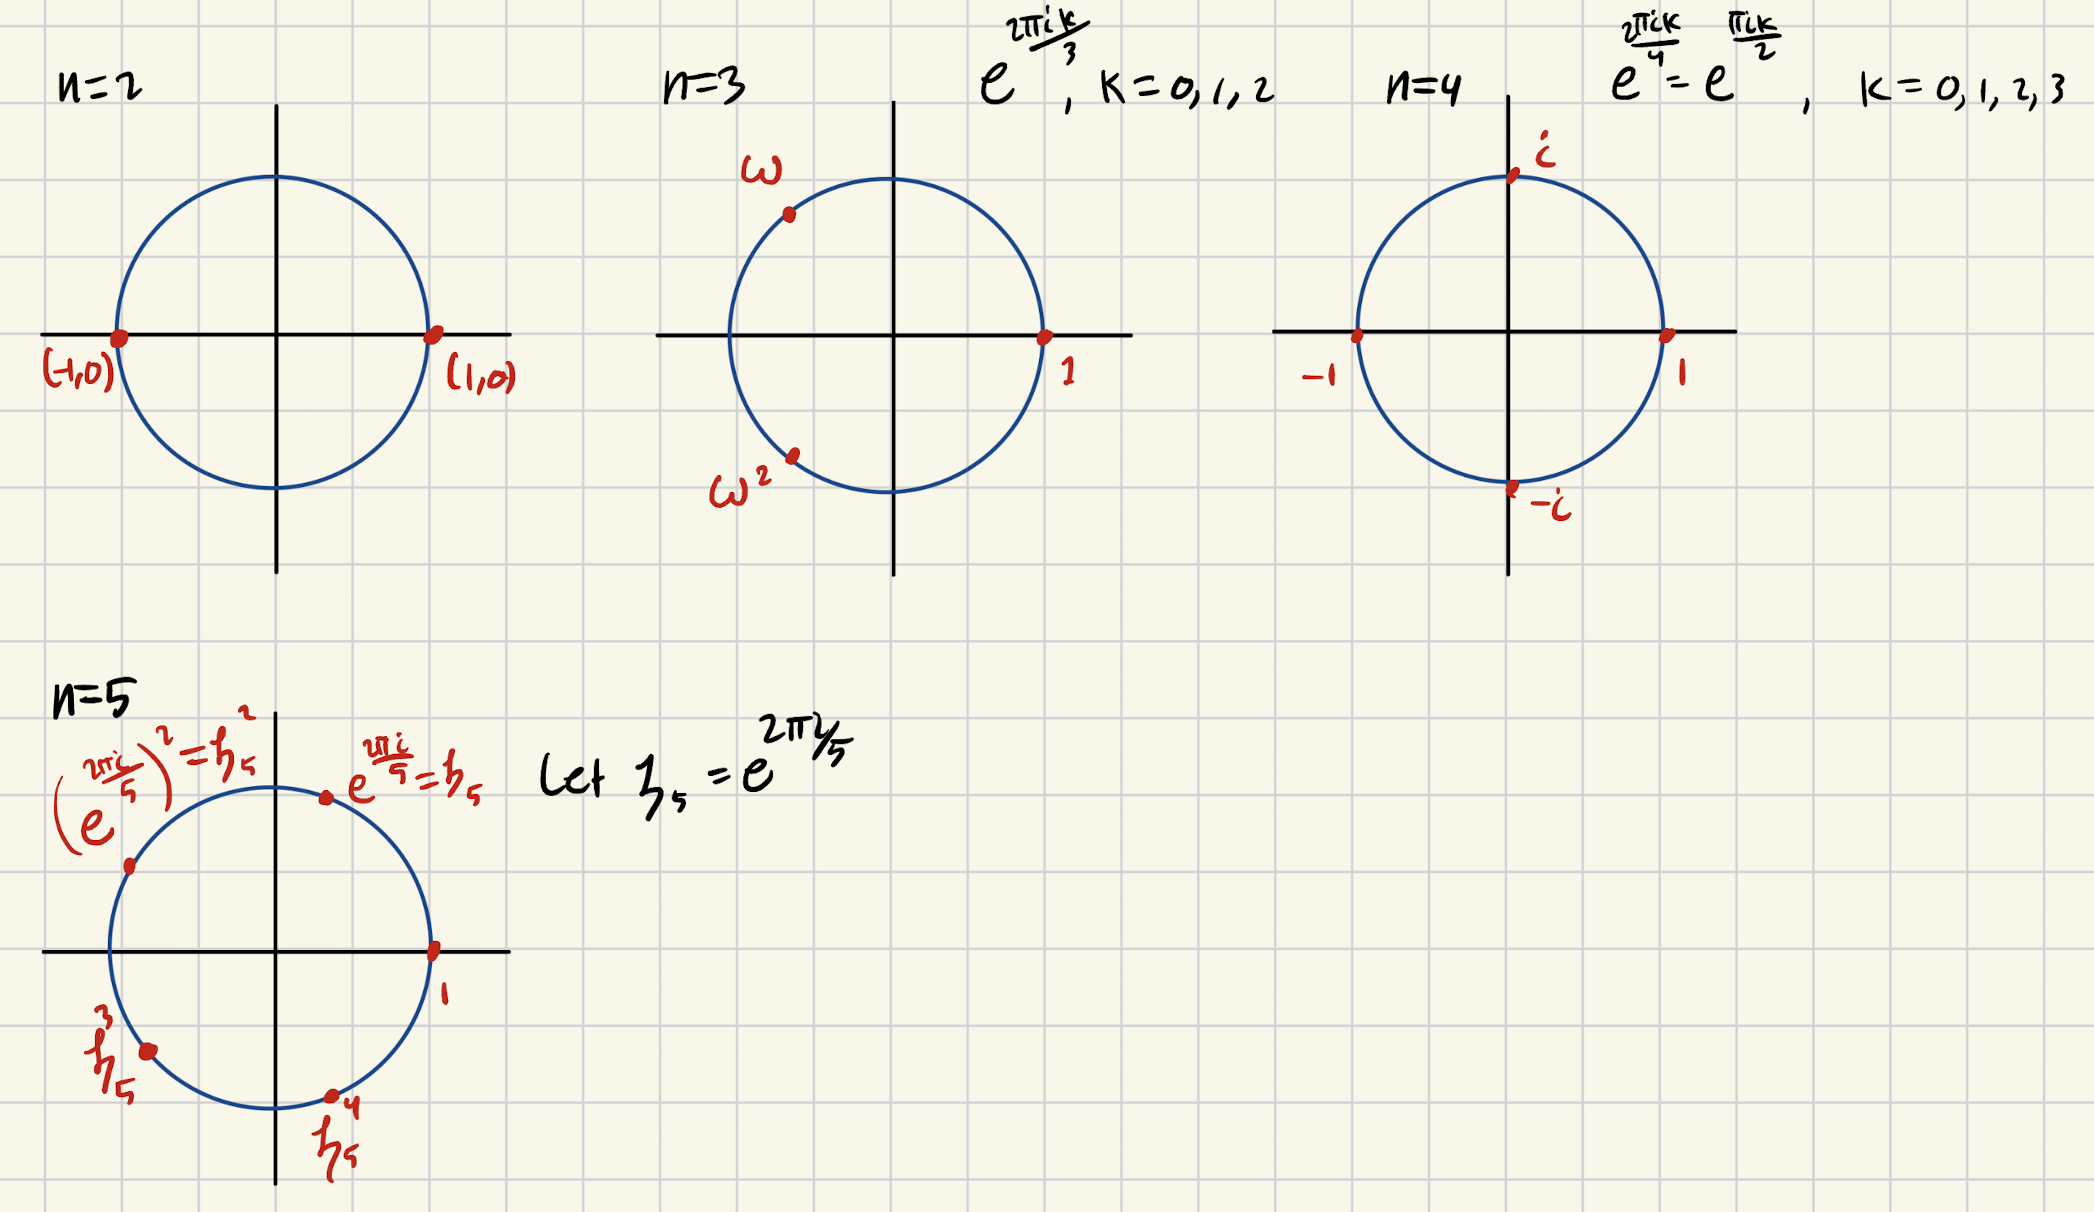
\includegraphics[width = 400pt, center]{CH4/images/Roots of Unity Circles.png}

Since $x^n - 1$ has at most $n$ roots in $\C$, it follows that all of the roots of $x^n -1$ are of the form $e^{\frac{2\pi i k}{n}}$ for $k = 0,1,..., n-1$. It's pretty easy to show $U_n$ is a group with respect to multiplication by constructing the following isomorphism:
\begin{align*}
    \quotient{\Z}{n\Z} &\to U_n \\
    k &\mapsto \left(e^{\frac{2 \pi i}{n}}\right)^k
\end{align*}
which would give us that $e^{\frac{2\pi i}{n}}$ is cyclic.

\begin{definition}[Primitive Root of Unity] \leavevmode \\
    A generator of $U_n$ is called a primitive root of unity.
\end{definition}

Let $\zeta$ be a primitive $n^\text{th}$-root of unity. Then
$$|\zeta |^k = \frac{n}{\gcd(n,k)}$$
Since $k = 0,1,...,n-1$, there are exactly $\phi(n)$ primitive $n^\text{th}$-roots of unity. Let $\zeta_n = e^{\frac{2\pi i}{n}}$. Some useful roots to know:
\begin{align*}
    \zeta_1 &= 1 \\
    \zeta_2 &= -1 \\
    \zeta_3 &= -\frac{1}{2} + \frac{\sqrt{3}}{2}i \\
    \zeta_4 &= i \\
    \zeta_5 &= \frac{\sqrt{5}-1}{4} + \frac{\sqrt{10+2\sqrt{5}}}{4}i \\
    \zeta_6 &= \frac{1}{2} + \frac{\sqrt{3}}{2}i \\ 
    \zeta_7 &= e^{\frac{2\pi i}{7}} \\
    \zeta_8 &= \frac{1}{\sqrt{2}} + \frac{1}{\sqrt{2}}i
\end{align*}

\begin{definition}[Cyclotomic Field] \leavevmode \\
    The field $\Q(\zeta_n)$ is called the cyclotomic field of $n^\text{th}$-roots of unity.
\end{definition}

Let $p$ be a prime.
\begin{align*}
    [\Q(\zeta_p) : \Q] &= p-1 \\
    x^p - 1 &= (x-1)(x^{p-1}+x^{p-2} + ... + x + 1) \\ 
    \implies \frac{x^p-1}{x-1} &= x^{p-1}+x^{p-2} + ... + x + 1
\end{align*}

We proved that $p(x) = \frac{x^p-1}{x-1}$ is irreducible ($p(x+1)$ with Eisenstein's Criterion). Since $\zeta_n \neq 1,$ $n > 1$ where $\zeta_n$ is a root of $p(x)$, so $m_{\zeta_n, \Q}(x) = p(x)$. In general,
$$[\Q(\zeta_n) : \Q] = \phi(n)$$

\begin{example}
    Find splitting field of $x^p - 2 = f(x) \in \Q[x]$, where $p$ is a prime. Note that the solutions to $f(x)$ are 
    $$\sqrt[p]{2} \zeta_p^k \text{ for } k= 0, 1, ..., p-1$$
    Let $K$ be the splitting field of $f(x)$ over $\Q$.
    $$K = \Q\left(\sqrt[p]{2}, \sqrt[p]{2}\zeta_p, \sqrt[p]{2}\zeta_p^2, ..., \sqrt[p]{2}\zeta_p^{p-1}\right)$$
    We know that $\sqrt[p]{2}, \sqrt[p]{2}\zeta_p \in K$. This implies
    $$\dfrac{\sqrt[p]{2}\zeta_p}{\sqrt[p]{2}} = \zeta_p \in K$$
    So, $K$ contains $\Q, \sqrt[p]{2}, \zeta_p$, so it contains $\Q(\sqrt[p]{2},\zeta_p)$. Note that since all the roots of $f(x)$ are of the form $\zeta_p^k \sqrt[p]{2},$ we have that all of $f(x)$'s roots are in $\Q(\sqrt[p]{2},\zeta_p)$. Hence
    $$K\subseteq \Q(\sqrt[p]{2},\zeta_p)$$
    So $K = \Q(\sqrt[p]{2},\zeta_p)$ and
    $$[K : \Q] = [K : \Q(\sqrt[p]{2})][\Q(\sqrt[p]{2}): \Q] \leq (p-1)p$$
    and $p \mid [K : \Q]$. Similarly, $p-1 \mid [K : \Q]$. Since $\gcd(p-1,p) = 1,$ we have that $p(p-1) \mid [K : \Q]$. Hence, $[K : \Q] = p(p-1)$.
\end{example}
\newpage

\section{Derivative of a Polynomial}
With splitting fields, we are able to factor polynomials into linear factors. Sometimes, these factors may repeat. For example, the polynomial $f(x) = (x-1)^2(x-2)$ has a repeated factor of $(x-1)$.

More generally, let $F$ be a field and $f(x) \in F[x]$. For $f(x)$, we have
$$f(x) = (x-\alpha_1)^{n_1}(x-\alpha_2)^{n_2}\cdots(x-\alpha_k)^{n_k}$$
where each $\alpha_i$ are distinct elements of $K$, a splitting field for $f(x)$ and $n_i \geq 1 \forall i$. $\alpha_i$ is called a repeated root if $n_i > 1$ where $n_i$ is the multiplcity of $\alpha_i$.

In calculus, we know that if $f(x)$ has a repeated root at $\alpha$, then $f'(\alpha) = 0$. We will make use of this idea to detect repeated roots of polynomials over fields.

\begin{definition}[Derivative of a Polynomial] \leavevmode \\
    Let $f(x) = \sum_{i=0}^n a_ix^i$ be a nonzero polynomial in $F[x]$. We define
    $$D_x f(x) = \sum_{i=1}^{n}a_{1}\cdot ix^{i-1} = a_1 + 2a_2x + \cdots + na_n x^{n-1}$$
    to be the formal derivative of $f(x)$.
\end{definition}

\begin{definition}[Separable Polynomial] \leavevmode \\
    A polynomial is separable if it has no multiple roots. A polynomial which is not separable is called inseparable.
\end{definition}

\begin{proposition}
    A polynomial $f(x)$ has a multiple root $\alpha$ if and only if $\alpha$ is also a root of $D_x f(x)$. I.e., $f(x)$ and $D_x f(x)$ are both divisible by the minimal polynomial of $\alpha$ over $F$. In particular, $f(x)$ is separable if and only if it is relatively prime to its derivative.
\end{proposition}

\begin{example}
    The product rule, power rule and chain rule hold with formal derivatives. That is,
    \begin{align*}
        D_x\left(f(x)g(x)\right)&= \left(D_xf(x)\right)g(x) + f(x)\left(D_x g(x)\right) \\ 
        D_x\left(\left(f(x)\right)^n\right) &= n\left(f(x)\right)^{n-1}D_x f(x) \\
        D_x \left((x-\alpha)^n\right) &= n (x-\alpha)^{n-1}
    \end{align*}
\end{example}

\begin{example}
    The polynomial $x^{p^n}-x$ over $\F_p$ has derivative 
    $$p^nx^{p^n-1} - 1 = 0 - 1 = -1 \text{ (using characteristic $p$)}$$
    so we can immediately see that $x^{p^n}-x$ is relatively prime to $D_x\left(x^{p^n-1}-x\right)$ and so $x^{p^n-1}-x$ is separable (it has no multiple roots).
\end{example}

\begin{corollary}
    Every irreducible polynomial over a field of characteristic $0$ is separable. A polynomial is separable if and only if it is the product of distinct irreducible polynomials.
\end{corollary}

\begin{proof}
    Suppose $\charc{F} = 0$ and $p(x) \in F[x]$ is irreducible of degree $n$. Then
    $$\deg \left(D_x\left(p(x)\right)\right) = n-1$$
    The only factors of the irreducible polynomial $p(x)$ are associates of $p(x)$ and associates of $1$ so $D_x(p(x))$ must be relatively prime to $p(x)$. Hence, $p(x)$ is separable.
    \qed
\end{proof}

\begin{proposition}
    Let $F$ be a field with $\charc{F} = p$ where $p$ is prime. Then for any $a,b \in F,$ $(a+b)^p = a^p+b^p$ and $(ab)^p = a^pb^p$. That is, the mapping defined by $\varphi(a) = a^p$ is an injective field homomorphism from $F$ to $F$ called the Frobenius automorphism.
\end{proposition}

\begin{example}
    Here is an important example. From homework, we proved that if $K/\F_p$ is finite then $|K| = p^n$ for some $n$. We will fix some $n \in \N$ and show there exists an extension $F/ \F_p$ such that $[F : \F_p] = n$.

    Let $n > 0$ and consider $f(x) = x^{p^n} - x \in \F_p[x]$. Let $K$ be the splitting field of $f(x)$ over $\F_p$. We know $f(x)$ is separable, thus it has exactly $p^n$ distinct roots. Let $\alpha, \beta$ be roots of $f(x)$. Then
    \begin{align*}
        \begin{rcases*}
            \alpha^{p^n}-\alpha = 0 \\
            \beta^{p^n}-\beta = 0
        \end{rcases*} \implies
        \begin{rcases*}
            \alpha^{p^n} = \alpha \\
            \beta^{p^n} = \beta
        \end{rcases*}
    \end{align*}
    Then
    \begin{align*}
        (\alpha \beta)^{p^n} &= \alpha^{p^n}\beta^{p^n} = \alpha \beta \\
        (\alpha^{-1})^{p^n} &= (\alpha^{p^n})^{-1} = \alpha^{-1} \\
        (\alpha + \beta)^{p^n} &= \alpha^{p^n} + \beta^{p^n} = \alpha + \beta
    \end{align*}
    Hence, the set of all $p^n$ roots of $f(x)$, $F$, is closed under addition, multiplication, and inverse in $K$. That is, $F$ is a subfield of $K$. Noting that $1\in F$, we see $\F_p \subseteq K$. Hence $K \subseteq F$, so $K=F$. Since $F$ is a vector space over $\F_p$ and $|F| = p^n$, it follows that $[F : \F_p] = n$. Hence, we have shown the existence of finite fields of order $p^n$.
\end{example}
\newpage

\chapter{Galois Theory}
\section{Field Automorphisms and Galois Groups}
After studying splitting fields, we are now in a position to study the symmetries of these fields. In particular, we will be interested in the field automorphisms of splitting fields. As we will see, automorphisms for splitting fields are closely tied to the roots of the polynomial that we are splitting. The collection of such automorphisms will form a group under composition, which will be known as the Galois group of the splitting field.

\begin{definition}[Field Automorphism] \leavevmode \\
    Let $L$ be a field.
    \begin{enumerate}
        \item A field isomorphism $\sigma: K \to K$ is called an automorphism of $K$. The set of all automorphisms of $K$ is denoted by $\Aut{K}$.
        \item We say $\sigma \in \Aut{K}$ fixes an element $\alpha \in K$ if $\sigma(\alpha) = \alpha$. If $F\subseteq K$, then $\sigma$ is said to fix $F$ if $\sigma(f) = f$ for all $f \in F$.
    \end{enumerate}
\end{definition}

\begin{example}
    $\sigma(a) = a ~~\forall a \in K$ is called the trivial automorphism (or the identity automorphism), denoted $\sigma_1$ or $1$.
\end{example}

\begin{note}
    The prime subfield of $K$, call it $F$ (for now) is generated by $1$ and since any automorphism $\tau$, $\tau(1)=1$, it follows that $\tau(a) = a$ for all $a\in F$. Hence any automorphisms of a field $K$ fixes its prime subfield. So, all $\tau \in \Q(\sqrt{2})$ fix $\Q$.
\end{note}

\begin{example}
    $\Aut{\Q} = \set{\sigma_1}$ since $\Q$ is its own prime subfield.
\end{example}

\begin{definition} [$\Aut{K/F}$] \leavevmode \\
    Let $K / F$ be an extension of fields. Let $\Aut{K/F}$ be the collection of automorphisms of $K$ which fix $F$.
\end{definition}

\begin{proposition}
    $\Aut{K}$ form a group with respect to composition and $\Aut{K/F}$ form a subgroup of $\Aut{K}$.
\end{proposition}

\begin{proof}
    Composition is an associative binary operation on bijective morphisms. The identity of $\Aut{K}$ is $\sigma_1$. Isomorphisms have functional inverses, which are isomorphisms. So, $\Aut{K}$ forms a group. Now, let $\sigma, \tau \in \Aut{K/F}$. Then let $a\in F$. We have 
    \begin{align*}
        \sigma \tau^{-1}(a) &= \sigma \tau^{-1}(\tau(a)) \\
        &= \sigma(a) \\
        &= a
    \end{align*}
    Hence, $\Aut{K/F} \leq \Aut{K}.$
    \qed
\end{proof}

\begin{proposition}
    Let $K/F$ be a field extension and let $\alpha \in K$ be algebraic over $F$. Then for any $\sigma \in \Aut{K / F}$, $\sigma(\alpha)$ is a root of the minimal polynomial for $\alpha$ over $F$. I.e., $\Aut{K / F}$ permutes the roots of irreducible polynomials. Equivalently, any polynomial in $F[x]$ which has $\alpha$ as a root will also have $\sigma(\alpha)$ as a root.
\end{proposition}

\begin{proof}
    If $\alpha$ satisfies $\sum_{i=0}^\infty a_i \alpha^i = 0$ where $a_i \in F$, then 
    \begin{align*}
        \sigma\left(\sum_{i=0}^\infty a_i \alpha^i\right) &= \sigma(0) \\
        \implies \sum_{i=0}^\infty \sigma(a_i \alpha^i) &= 0 \\
        \implies \sum_{i=0}^\infty \sigma(a_i) \sigma(\alpha^i) &= 0 \\
        \implies \sum_{i=0}^\infty a_i \sigma(\alpha^i) &= 0
    \end{align*}
    \qed
\end{proof}

\begin{example}
    Consider $K = \Q(\sqrt{2})$. If $\tau \in \Aut{K} = \Aut{K/Q}$, then $\tau(\sqrt{2}) = \pm \sqrt{2}$ since $\pm \sqrt{2}$ are the two roots of $m_{\sqrt{2}, \Q}(x)$. We have two possible automorphisms:
    \begin{align*}
        1: \sqrt{2} &\mapsto \sqrt{2} \\
        \sigma : \sqrt{2} &\mapsto -\sqrt{2}
    \end{align*}
    Note $\sigma^2$:
    \begin{align*}
        \sigma^2(\sqrt{2}) &= \sigma(-\sqrt{2}) \\
        &= -\sigma(\sqrt{2}) \\
        &= -(-\sqrt{2}) \\ 
        &= \sqrt{2} \\
        \implies \sigma^2 &= 1
    \end{align*}
    Then $\Aut{\Q(\sqrt{2})/\Q} = \cyc{\sigma} \cong \quotient{\Z}{2\Z}$.
\end{example}

\begin{example}
    Consider $\Q(\sqrt[3]{2})$. If $\tau \in \aut{K}$, we have the following possibilities: $\tau \in (\sqrt[3]{2}) \in \set{\sqrt[3]{2}, \sqrt[3]{2}\omega, \sqrt[3]{2}\omega^2}$ since $m_{\sqrt[3]{2}, \Q}(x) = x^3 -2.$ Since $\Q(\sqrt[3]{2}) \subseteq \R$, $\tau$ cannot map to  $\sqrt[3]{2}\omega, \sqrt[3]{2}\omega^2 \in \C$. Hence $\tau(\sqrt[3]{2}) = \sqrt[3]{2}$ ($\tau = 1$). Thus there is only one automorphism of $\Q(\sqrt[3]{2})$, namely $1$. Hence, $\aut{\Q(\sqrt[3]{2}) / \Q} = 1.$
\end{example}
Comparing $\aut{\Q(\sqrt{2})}$ and $\aut{\Q(\sqrt[3]{2})}$, we see that $\aut{\Q(\sqrt[3]{2})}$ is missing clear automorphisms. In general, we see that if $K/F$ is generated by some collection of elements, then $\sigma \in \aut{K/F}$ is completely determined by where $\sigma$ maps the generators.

\begin{proposition}
    Let $H \leq \aut{K}$. Then the elements of $K$ fixed by all automorphisms in $H$ is a subfield of $K$.
\end{proposition}

\begin{proof}
    Let $h \in H$, $a,b\in F$. Then, by definition, $h(a) = a$ and $h(b) = b$ so that 
    $$h(a\pm b) = h(a) \pm h(b).$$
    Further,
    $$h(ab) = h(a)h(b)$$
    and
    $$h(a^{-1}) = h(a)^{-1} = a^{-1}$$
    Thus, $F$ is a field.
    \qed
\end{proof}

\begin{note}
    $H$ does not have to be a subgroup for the proposition to hold.
\end{note}

We the above proposition, we take interest in the elements in $K$ that are fixed by the automorphisms of $K$.

\begin{definition}[Fixed Field] \leavevmode \\
    If $H \leq \aut{K}$, the subfield fixed by $H$ is called the fixed field of $H$.
\end{definition}

\begin{proposition}
    The association of groups of $\aut{K}$ to fixed fields and fixed fields to subgroups is inclusion reversing. Namely,
    \begin{enumerate}
        \item If $F_1 \subseteq F_2 \subseteq K$ are subfields of $K$, then $\aut{K/F_2} \subseteq \aut{K /F_1}$.
        \item If $H_1 \leq H_2 \leq \aut{K}$ where $F_1$ and $F_2$ are the associated fixed fields of $H_1$ and $H_2$, respectively, then $F_1 \subseteq F_2$.
    \end{enumerate}
\end{proposition}

\begin{proof}
    \begin{enumerate}
        \item Let $\sigma \in \aut{K/ F_2}$. Let $a \in F_1$. Then $a \in F_2$ so 
        $$\sigma(a) = a$$
        Hence, $\sigma$ fixes $F_1$ and 
        $$\aut{K/F_2} \subseteq \aut{K/F_1}$$

        \item Let $\sigma \in H_1.$ Let $a \in F_1$. Since $H_1 \subseteq H_2$, $\sigma \in H_2$ so
        $$a = \sigma(a) \in F_2$$
    \end{enumerate}
\end{proof}

\begin{example}
    Let $K = \Q(\sqrt{2})$. Then the fixed field of 
    $$\aut{\Q(\sqrt{2})} = \aut{\Q(\sqrt{2})/\Q} = \set{1, \sigma}$$
    is the set of all $a+b\sqrt{2} \in \Q(\sqrt{2})$ such that 
    \begin{align*}
        1(a + b\sqrt{2}) &= a + b\sqrt{2} \\
        \sigma(a + b\sqrt{2}) &= a + b\sqrt{2}
    \end{align*}
    Thus, we must have that 
    \begin{align*}
        a-b\sqrt{2} &= a+b\sqrt{2} \\
        \implies -b\sqrt{2} &= b\sqrt{2} \\
        \implies -b &= b \\
        \implies b &= 0
    \end{align*}
    So, the fixed field of $\aut{\Q(\sqrt{2})/\Q}$ is just $\Q$.
\end{example}

\begin{example}
    Let $K = \Q(\sqrt{2})$. The fixed field of $\aut{\Q(\sqrt[3]{2})/\Q} = 1$ is $Q(\sqrt[3]{2})$. Notice that for $\Q(\sqrt{2})$ we have

    \begin{center}
        \begin{tabular}{ccc}
            % Header Row
            \textbf{Subgroups of $\aut{\Q({\sqrt{2}})/\Q}$:} & & \textbf{Fixed fields:} \\ 
            \noalign{\medskip} % Adds a bit more space after the header
            
            % Data Row
            $\set{1}$ & $\longleftrightarrow$ & $\Q(\sqrt{2})$ \\
            $\set{1, \sigma}$ & $\longleftrightarrow$ & $\Q$
        \end{tabular}
    \end{center}

    With $\Q(\sqrt[3]{2})$, we have 
    \begin{center}
        \begin{tabular}{ccc}
            % Header Row
            \textbf{Subgroups of $\aut{\Q({\sqrt{2}})/\Q}$:} & & \textbf{Fixed fields:} \\ 
            \noalign{\medskip} % Adds a bit more space after the header
            
            % Data Row
            $\set{1}$ & $\longleftrightarrow$ & $\Q(\sqrt[3]{2})$
        \end{tabular}
    \end{center}
    but we have no set of automorphisms which fix $\Q$.
\end{example}

\begin{proposition}
    Let $E$ be the splitting field over $F$ of some polynomial $f(x) \in F[x]$. Then
    $$|\aut{E/F}| \leq [E:F]$$
    with equality when $f(x)$ is separable over $F$.
\end{proposition}

\begin{definition}[Galois Extensions and Groups] \leavevmode \\
    Let $K/F$ be a finite extension. Then $K$ is said to be Galois over $F$ ($K/F$ is a Galois Extension) if $|\aut{K/F}| = [K:F]$. If $K/F$ is Galois, the group of automorphisms $\aut{K/F}$ is called the Galois group of $K/F$, denoted $\Gal{K/F}$.
\end{definition}

\begin{corollary}
    If $K$ is the splitting field over $F$ of a separable polynomial $f(x)$, then $K/F$ is Galois.
\end{corollary}

\begin{definition}[Galois Group of a Polynomial] \leavevmode \\
    If $f(x)$ is a separable polynomial over $F$, then the Galois group of $f(x)$ over $F$ is $\Gal{K/F}$ where $K$ is the splitting field of $f(x)$ over $F$.
\end{definition}

\begin{example}
    Show $\Q(\sqrt{2})/\Q$ is Galois. \\
    We know that $[\Q(\sqrt{2}):\Q] = 2$ and that $\aut{\Q(\sqrt{2})/\Q} = \set{1, \sigma}$. Hence, $\Q(\sqrt{2})/\Q$ is a Galois extension.

    Alternatively, we know that $\Q(\sqrt{2})$ is the splitting field of $x^2-2 \in \Q[x]$. Hence, $\Q(\sqrt{2})$ is Galois over $\Q$.
\end{example}

\begin{example}
    The extension $\Q(\sqrt[3]{2})/\Q$ is not Galois since
    $$[\Q(\sqrt[3]{2}):\Q] = 3 \text{ but } \aut{\Q(\sqrt[3]{2})/\Q} = 1$$
\end{example}

\begin{example}
    The extension $\Q(\sqrt{2}, \sqrt{3})$ is Galois since it is the splitting field of the separable polynomial $(x^2-2)(x^2-3) \in \Q [x]$. Calculating the Galois group:
    
    Any $\sigma \in \Gal{\Q(\sqrt{2},\sqrt{3})/\Q}$ can be determined by its action on $\sqrt{2}$ and $\sqrt{3}$. We know that $\sqrt{2}$ and $\sqrt{3}$ must map to $\pm \sqrt{2}$ and $\pm \sqrt{3}$, respectively. Hence, the only possible automorphisms are
    \begin{center}
        \begin{tabular}{cc}
            % Data Row
            $\begin{cases*}
                \sqrt{2} \mapsto \sqrt{2} \\
                \sqrt{3} \mapsto \sqrt{3}
            \end{cases*}$ & 
            $\begin{cases*}
                \sqrt{2} \mapsto -\sqrt{2} \\
                \sqrt{3} \mapsto \sqrt{3}
            \end{cases*}$ \\
            $\begin{cases*}
                \sqrt{2} \mapsto \sqrt{2} \\
                \sqrt{3} \mapsto -\sqrt{3}
            \end{cases*}$ &
            $\begin{cases*}
                \sqrt{2} \mapsto -\sqrt{2} \\
                \sqrt{3} \mapsto -\sqrt{3}
            \end{cases*}$
        \end{tabular}
    \end{center}
    Let
    \begin{align*}
        \sigma = 
        \begin{cases*}
            \sqrt{2} \mapsto -\sqrt{2} \\
            \sqrt{3} \mapsto \sqrt{3}
        \end{cases*}, ~~\tau = 
        \begin{cases*}
            \sqrt{2} \mapsto \sqrt{2} \\
            \sqrt{3} \mapsto \sqrt{3}
        \end{cases*}
    \end{align*}
    Notice
    $$\sigma^2(\sqrt{2}) = \sqrt{2} \text{ and } \sigma^2(\sqrt{3}) = \sqrt{3} \implies \sigma^2 = 1$$
    Similarly, $\tau^2 = 1$. Furthermore,
    $$\sigma(\tau(\sqrt{2})) = -\sqrt{2}, ~~\sigma(\tau(\sqrt{3}))=-\sqrt{3}$$
    so
    $$
    \sigma \tau = \begin{cases*}
        \sqrt{2} \mapsto -\sqrt{2} \\
        \sqrt{3} \mapsto -\sqrt{3}
    \end{cases*}
    $$
    Lastly, $\sigma \tau = 1$ so 
    $$\Gal{\Q(\sqrt{2}, \sqrt{3})/\Q} \cong \Z_2 \times \Z_2$$
\end{example}

\begin{example} Let's look at the corresponding fixed fields of the previous example.

    \begin{center}
        \begin{tabular}{ccc}
            \textbf{Subgroups of $\Gal{\Q({\sqrt{2}}, \sqrt{3})/\Q}$:} & & \textbf{Corresponding fixed fields:} \\ 
            \noalign{\medskip}
            % Data Row
            $1$ & $\longleftrightarrow$ & $\Q(\sqrt{2}, \sqrt{3})$ \\
            $\cyc{\sigma}$ & $\longleftrightarrow$ & $\Q(\sqrt{3})$ \\
            $\cyc{\tau}$ & $\longleftrightarrow$ & $\Q(\sqrt{2})$ \\
            $\cyc{\sigma \tau}$ & $\longleftrightarrow$ & $\Q(\sqrt{6})$ \\ 
            $\set{1, \sigma, \tau, \sigma \tau}$ & $\longleftrightarrow$ & $\Q$
        \end{tabular}
    \end{center}
    To find the fixed field for $\cyc{\sigma}$, note that
    \begin{align*}
        \sigma(a+b\sqrt{2}+c\sqrt{3}+d\sqrt{6}) &= a + b\sigma(\sqrt{2})+c\sigma(\sqrt{3})+d\sigma(\sqrt{6}) \\
        &= a-b\sqrt{2}+c\sqrt{3}+d\sigma(\sqrt{2})\sigma(\sqrt{3}) \\
        &= a-b\sqrt{2}+c\sqrt{3}-d\sqrt{6}
    \end{align*}
    An element in $\Q(\sqrt{2}, \sqrt{3})$ is fixed by $\sigma$ if 
    \begin{align*}
        a+b\sqrt{2} + c\sqrt{3} + d\sqrt{6} &= a-b\sqrt{2}+c\sqrt{3}-d\sqrt{6} \\
        \implies b=-b &\text{ and } d = -d \\
        \implies b=&d=0
    \end{align*}
    so $\sigma(a+b\sqrt{2}+c\sqrt{3}+d\sqrt{6}) = a+c\sqrt{3} \in \Q(\sqrt{3})$.

    Similarly, for $\cyc{\tau},$
    \begin{align*}
        \tau(a+b\sqrt{2}+c\sqrt{3}+d\sqrt{6}) &= a + b\sqrt{2}-c\sqrt{3}-d\sqrt{6} \\
        \implies c = &0 = d \\
        \implies \tau(a+b\sqrt{2}+c\sqrt{3}+d\sqrt{6})&= a + b\sqrt{2} \in \Q(\sqrt{2})
    \end{align*}
\end{example}

\begin{example}
    Let $p(x) = x^3-2 \in \Q[x]$. We have found the splitting field of $p(x)$ over $\mathbb{Q}$ to be $\Q(\sqrt[3]{2}, \omega)$ where $\omega = \frac{-1+\sqrt{3}i}{2}.$

    Notice that $x^3-2$ has three distinct roots, so $p(x)$ is separable and so its splitting field is Galois over $\Q$. We also know
    $$[\Q(\sqrt[3]{2}, \omega):\Q] = 6 = \left| \Gal{\Q(\sqrt[2]{3}, \omega)/\Q}\right|.$$
    Suppose we write the splitting field as
    $$\Q(\sqrt[3]{2}, \sqrt[3]{2}\omega)$$
    We know that any automorphism will send roots of minimal polynomials to other roots. Written this way, we may have 
    \[
        \begin{tikzcd}[column sep=large]
            & \sqrt[3]{2} \\
            \sqrt[3]{2} \arrow[ru, mapsto] \arrow[r, mapsto] \arrow[rd, mapsto] & \sqrt[3]{2} \omega \\
            & \sqrt[3]{2} \omega^2
        \end{tikzcd}, 
        \begin{tikzcd}[column sep=large]
            & \sqrt[3]{2} \\
            \sqrt[3]{2}\omega \arrow[ru, mapsto] \arrow[r, mapsto] \arrow[rd, mapsto] & \sqrt[3]{2} \omega \\
            & \sqrt[3]{2} \omega^2
        \end{tikzcd}
    \]

    This gives $3 \cdot 3 = 9$ possibilities for automorphisms, which is larger than the order of the Galois group. 

    Using $\Q(\sqrt[3]{2}, \omega)$, we have a more compatible number of potential automorphisms. Any automorphism can send
        \[
        \begin{tikzcd}[column sep=large]
            \omega \arrow[r, mapsto] \arrow[rd, mapsto] & \omega \\
             & \omega^2
        \end{tikzcd}, 
        \begin{tikzcd}[column sep=large]
             & \sqrt[3]{2} \\
            \sqrt[3]{2} \arrow[ru, mapsto] \arrow[r, mapsto] \arrow[rd, mapsto] & \sqrt[3]{2} \omega \\
            & \sqrt[3]{2} \omega^2
        \end{tikzcd}
    \]
    ($m_{\omega, \Q}(x) = x^2 + x + 1$, $m_{\sqrt[3]{2}, \Q}(x) = x^3-2$).
    This gives six automorphisms, which is exactly the size of the Galois group. Let
    \begin{align*}
        1 &: \begin{cases*}
            \sqrt[3]{2} \mapsto \sqrt[3]{2} \\
            \omega \mapsto \omega
        \end{cases*} \\
        \sigma &: \begin{cases*}
            \sqrt[3]{2} \mapsto \sqrt[3]{2}\omega \\
            \omega \mapsto \omega
        \end{cases*} &&
        \tau: \begin{cases*}
            \sqrt[3]{2} \mapsto \sqrt[3]{2} \\
            \omega \mapsto \omega^2 = -1-\omega
        \end{cases*}
    \end{align*}
    \begin{align*}
                \sigma^2 &: \begin{cases*}
            \sqrt[3]{2} \mapsto \sigma(\sqrt[3]{2}\omega) \mapsto \sqrt[3]{2}\omega^2 = \sqrt[3]{2}(-1-\omega) \\
            \omega \mapsto \omega
        \end{cases*} &&
        \tau^2: \begin{cases*}
            \sqrt[3]{2} \mapsto \sqrt[3]{2} \\
            \omega \mapsto \left(\omega^2\right)^2 = \omega^4 = \omega
        \end{cases*} \\
        \sigma^3 &: \begin{cases*}
            \sqrt[3]{2} \mapsto \sqrt[3]{2}\omega(-1-\omega) = \sqrt[3]{2}(-\omega + 1 + \omega) = \sqrt[3]{2} \\
            \omega \mapsto \omega
        \end{cases*}
    \end{align*}
    Notice that $\sigma^3 = 1 = \tau^2$, so $|\sigma| = |\cyc{\sigma}| = 3$ and $|\tau| = |\cyc{\tau}| = 2$.

    \begin{align*}
        \sigma \tau &: \begin{cases*}
            \sqrt[3]{2} \mapsto \sqrt[3]{2} \omega \\
            \omega \mapsto -1-\omega
        \end{cases*} &&
        \tau \sigma: \begin{cases*}
            \sqrt[3]{2} \mapsto \sqrt[3]{2}(-1-\omega) \\
            \omega \mapsto (-1-\omega)
        \end{cases*}
    \end{align*}
    $\omega \tau \neq \tau \omega,$ so the Galois group is not abelian.
    \begin{align*}
        \tau\sigma^2 &: \begin{cases*}
            \sqrt[3]{2} \mapsto \sqrt[3]{2}\omega \\
            \omega \mapsto -1-\omega
        \end{cases*}
    \end{align*}
    $$\sigma\tau = \tau \sigma^2 \iff \sigma \tau = \tau \sigma^{-1}$$
    Hence,
    $$\Gal{\Q(\sqrt[3]{2}, \omega)/\Q} \cong \cyc{\sigma, \tau : \sigma^3 = \tau^2 = 1, \sigma \tau = \tau \sigma^{-1}} \cong D_6$$
\end{example}

\begin{example}
    Let's compute the fixed field of $\cyc{\sigma}$ from the previous example.

    We need to see what is fixed by the generator $\sigma$. Lets look at the basis for $\Q(\sqrt[3]{2}, \omega)$:
    $$\set{1, \sqrt[3]{2}, \left(\sqrt[3]{2}\right)^2, \omega, \sqrt[3]{2}\omega, \left(\sqrt[3]{2}\right)^2\omega}.$$
    Then,
    \begin{align*}
        \sigma(1) &= 1 \\
        \sigma\left(\sqrt[3]{2}\right) &= \sqrt[3]{2}\omega \\
        \sigma\left((\sqrt[3]{2}) ^2\right) &= \sigma\left(\sqrt[3]{2}\right)\sigma\left(\sqrt[3]{2}\right) = \left(\sqrt[3]{2}\omega\right)\left(\sqrt[3]{2}\omega\right) = \sqrt[3]{4}(-1-\omega) \\
        \sigma(\omega) &= \omega \\
        \sigma\left(\sqrt[3]{2} \omega\right) &= \sigma\left(\sqrt[3]{2}\right)\sigma(\omega) = \left(\sqrt[3]{2} \omega\right)\left(\omega\right) = \sqrt[3]{2}(-1-\omega) \\
        \sigma\left((\sqrt[3]{2})^2 \omega\right) &= \sigma\left((\sqrt[3]{2})^2\right)\sigma(\omega) = \left(\sqrt[3]{4}(-1-\omega)\right)(\omega) = \sqrt[3]{4}(-\omega + 1 + \omega) = \sqrt[3]{4}
    \end{align*}
    So,
    \begin{align*}
        \sigma\left(a+b\sqrt[3]{2} + c(\sqrt[3]{2})^2+d\omega + e\sqrt[3]{2} \omega + f (\sqrt[3]{2})^2 \omega\right)
        &= a + b \sqrt[3]{2} \omega + c \left((\sqrt[3]{2})^2\omega^2\right) + dw + e\sqrt[3]{2} \omega^2 + f (\sqrt[3]{2})^2 \\
        &= a + b \sqrt[3]{2} \omega - c(\sqrt[3]{2})^2(1+\omega) + d\omega - e \sqrt[3]{2}(1+w) + f(\sqrt[3]{2})^2 \\
        &= a - e \sqrt[3]{2} + (f-c)(\sqrt[3]{2})^2 +d\omega + (b-e)\sqrt[3]{2} \omega -c (\sqrt[3]{2})^2 \omega
    \end{align*}
    For our element to be fixed, we need
    \begin{align*}
        &a = a &&f=-c \\
        &b=-e &&c=f-c \\
        &d=d &&e=b-e
    \end{align*}
    We have
    $$e=b-e = -e-e \implies e = 0 \implies b = 0$$
    Similarly,
    $$c=0 \implies f = 0$$
    Hence, any elements fixed by $\sigma$ are of the form $a + dw$. The fixed field of $\cyc{\sigma}$ is $\Q(\omega)$.
\end{example}

\begin{example}
    $\Q(\sqrt{2}, \sqrt[3]{3}, \sqrt[5]{5},...) = \bigcap \limits_{\substack{F \supseteq \Q \\ \sqrt[p_i]{p_i} \in F}} F$
    Note that
    $$\bigcap_{\substack{F \supseteq \Q \\ \sqrt[p_i]{p_i} \in F}} F = \bigcup_{i=1}^\infty K_i \text{ where } K_i = \Q\left(\sqrt[2]{2}, \sqrt[3]{3}, \sqrt[5]{5},...,\sqrt[p_i]{p_i}\right)$$
\end{example}
\newpage

\section{The Fundamental Theorem of Galois Theory}
Previously, we found the splitting field for $x^3-2,$ $K=\Q(\sqrt[3]{2}, \omega)$, and we calculated $\Gal{\Q(\sqrt[3]{2}, \omega)/\Q}$. We also looked at subfields of $\Q(\sqrt[3]{2}, \omega)$:

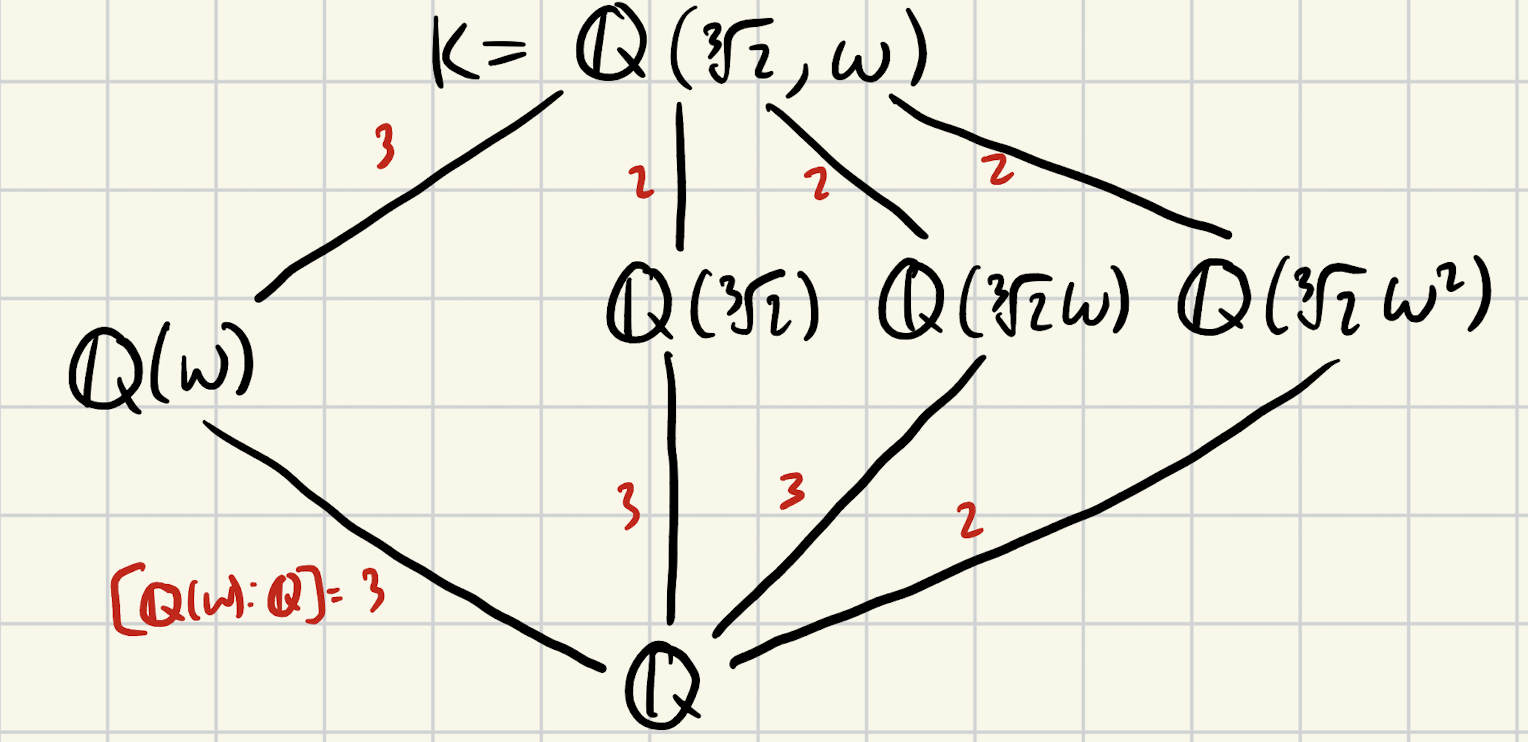
\includegraphics[width=350pt, center]{CH5/images/Subfield Lattice 1.png}

The subgroup lattice of the Galois group $K$ over $\Q$:

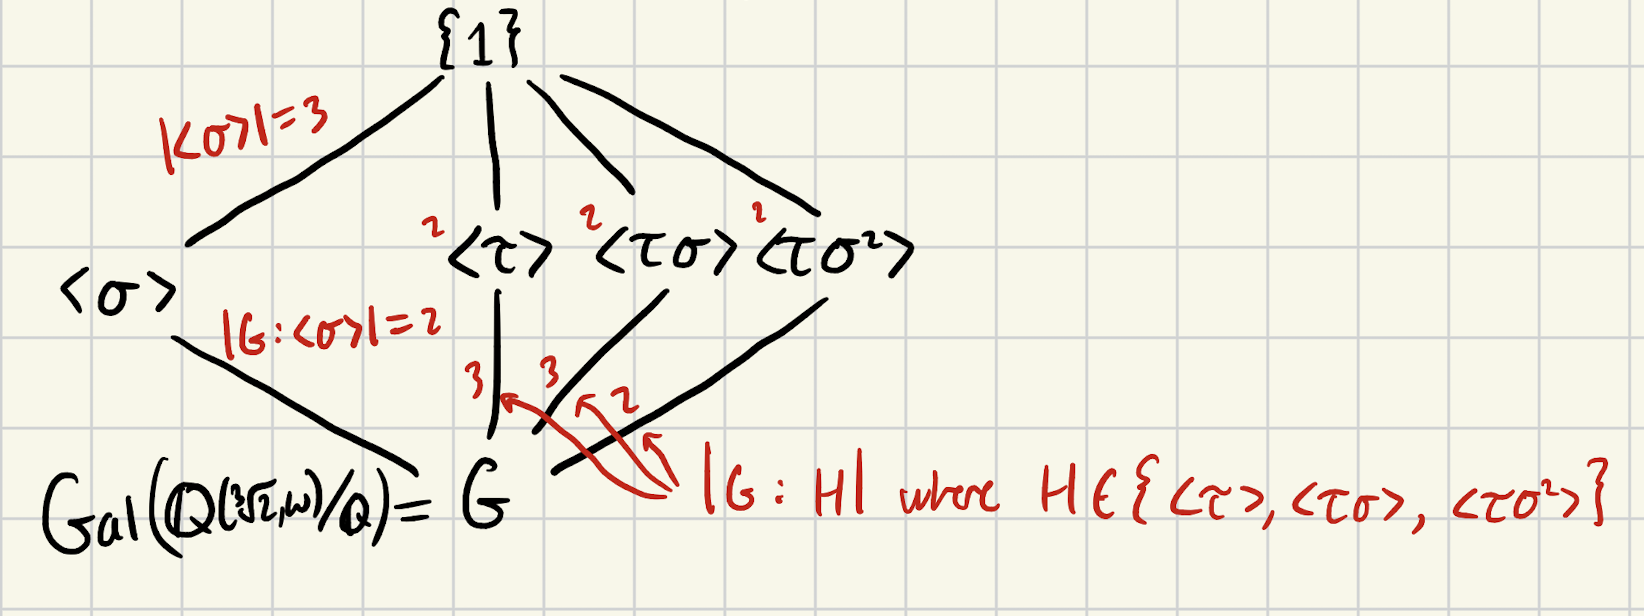
\includegraphics[width=350pt, center]{CH5/images/Subgroup Lattice 1.png}

\begin{theorem}[The Fundamental Theorem of Galois Theory] \leavevmode \\
    Let $K/F$ be a Galois extension and set $G = \Gal{K/F}$. Then there is a bijection between the set of subfields $E$ of $K$ containing $F$ and the subgroups of $G$
    $$
        \begin{tikzcd}[column sep=small]
            K \arrow[d, dash] \\
            E \arrow[d, dash] \\
            F
        \end{tikzcd}
        \longleftrightarrow
        \begin{tikzcd}[column sep=small]
            1 \arrow[d, dash] \\
            H \arrow[d, dash] \\
            G
        \end{tikzcd}
    $$
    given by the correspondence
    \begin{align*}
        E &\rightarrow \set{\text{the elements of $G$ fixing $E$}} \\
        \set{\text{The fixed field of $H$}} &\leftarrow H
    \end{align*}
    which are inverses to each other. Under this correspondence, we have the following results:
    \begin{enumerate}
        \item (Inclusion Reversing) If $E_1, E_2$ correspond to $H_1$ and $H_2$, respectively, then
        $$E_1 \subseteq E_2 \iff H_2 \subseteq H_1$$
        \item $[K:E] = |H|$ and $[E:F] = |G:H|$
        $$
        \begin{tikzcd}[column sep=large, row sep=large]
            K \arrow[d, dash, "\left. \rule{0pt}{2.5ex} \right\} |H|" right] \\
            E \arrow[d, dash, "\left. \rule{0pt}{2.5ex} \right\} |G:H|" right] \\
            F
        \end{tikzcd}
        $$
        \item The extension $K/E$ is always Galois with $\Gal{K/E}=H$.
        $$
        \begin{tikzcd}[column sep=large, row sep=large]
            K \arrow[d, dash, "\textstyle \quad H" right] \\
            E
        \end{tikzcd}
        $$
        \item $E$ is Galois over $F$ if and only if $H$ is a normal subroup of $G$. If this is the case, then the Galois group of $E$ over $F$ is isomorphic to the quotient group $\quotient{G}{H}$. That is,
        $$\Gal{E/F} \cong \quotient{G}{H}$$
        \item If $E_1, E_2$ correspond to $H_1, H_2,$ respectively, then $E_1 \cap E_2$ corresponds to the group $\cyc{H_1, H_2}$ and $E_1E_2$ corresponds to $H_1 \cap H_2$.
    \end{enumerate}
\end{theorem}

\begin{example}
    Let $p(x) = x^8-2$. Find the Galois group of the splitting field of $p(x)$ over $\Q$. The zeros of $p(x)$ are:
    $$\theta, \theta \zeta, \theta \zeta^2, \theta \zeta^3, ..., \theta \zeta^7 \text{ where } \zeta = \zeta_8, ~~ \theta = \sqrt[8]{2}$$
    Hence, $\theta, \theta \zeta \in K.$ Thus
    \begin{align*}
        \zeta = \dfrac{\theta \zeta}{\theta} &\in K \\
        \implies \Q(\theta, \zeta) &\subseteq K
    \end{align*}
    Further, each root of $p(x)$ can be constructed with $\theta$ and $\zeta$. Hence, $\theta \zeta^n \in \Q(\theta, \zeta)$ for all $n=0,1,..., 7.$ This gives $K \subseteq \Q(\theta, \zeta)$. Hence, $K = \Q(\theta, \zeta)$. We know $\zeta = \frac{1}{\sqrt{2}} + \frac{1}{\sqrt{2}}i,$ thus
    \begin{align*}
        \Q(\zeta) = \Q(i, \sqrt{2}) \\ 
        \left(\zeta + \zeta^7 = \sqrt{2}, ~~\zeta^2 = i\right)
    \end{align*}
    So, $K=\Q(\theta, i, \sqrt{2})$. But $\theta^4 = \sqrt{2}$, so $K = \Q(\theta, i)$ since $x^8-2$ is irreducible over $\Q$ by Eisenstein's. We have
    $$[\Q(\theta) : \Q] = 8$$
    and since $x^2+1$ is irreducible over $\Q$ with roots $\pm i$
    $$[\Q(i) : \Q] = 2$$
    so
    \begin{align*}
        [K : \Q] &\leq 2 \cdot 8 = 16 \\
        [K : \Q] &= [K : \Q(\theta)][\Q(\theta) : \Q]
    \end{align*}
    However, $K \neq \Q(\theta)$ since $\Q(\theta) \subseteq \R$ but $i \not \in \R$. Thus
    $$[K : \Q(\theta)] = 2$$
    It follows that $[K : \Q] = 16.$ Thus $G = \Gal{K/\Q}$ has order $16$. The possible automorphisms are
    $$\begin{cases*}
        \theta \mapsto \theta \zeta^a \\
        i \mapsto \pm i
    \end{cases*} \text{ where } a = 0,1,..., 7$$
    Define
    \begin{align*}
        \sigma: &\begin{cases*}
            \theta \mapsto \theta \zeta \\
            i \mapsto i
        \end{cases*} &&
        \tau: \begin{cases*}
            \theta \mapsto \theta \\
            i \mapsto -i
        \end{cases*} \\
        &(\zeta \mapsto \zeta^5)
        &&(\zeta \mapsto \bar{\zeta} = \zeta^7)
        \tag{$*$} \\
        \sigma^2: &\begin{cases*}
            \theta \mapsto \sigma(\theta \zeta) = \theta \zeta \cdot \theta^5 = \theta \zeta^6 \\
            i \mapsto i
        \end{cases*} \\
        &\vdots
    \end{align*}
    Continuing, we get $|\sigma| = 8$ and $|\tau| = 2.$ The group is 
    $$\set{1, \sigma, \sigma^2, ..., \sigma^7, \tau, \tau \sigma, ..., \tau \sigma^7}$$
    with $\sigma \tau = \tau \sigma^3.$ Thus
    $$G = \cyc{\tau, \sigma : \tau^2 = \sigma^8 = 1, \sigma \tau = \tau \sigma^3}$$
    This is a quasi-dihedral group.

    ($*$) Notice 
    \begin{align*}
        \sigma(\sqrt{2}) &= \sigma(\theta^4) \\
        &= \sigma(\theta)^4 \\
        &= \left(\theta \zeta\right)^4 \\
        &= \theta^4 \zeta^4 \\
        &= \theta^4(-1) \\
        &= -\sqrt{2}
    \end{align*} and so 
    \begin{align*}
        \zeta = \dfrac{1+i}{\sqrt{2}}, ~~\sigma(\zeta) = \dfrac{1+i}{-\sqrt{2}} = -\zeta = \zeta^5
    \end{align*}
\end{example}
\newpage

\end{document}